% ══════════════════════════════════════════════════════════════════════════════
% VERSÃO NORMATIVA — MBA USP/Esalq (Manual de Instruções e Normas, itens 15–19)
% Gerada por tcc/scripts/gerar_tcc_normas.py. NÃO editar à mão.
% ══════════════════════════════════════════════════════════════════════════════
\documentclass[11pt, a4paper, oneside]{article}
\usepackage[utf8]{inputenc}
\usepackage[T1]{fontenc}
\usepackage[brazil]{babel}
% termos estrangeiros nao devem ser hifenizados pelas regras do portugues
\hyphenation{Scien-ce Ana-ly-tics boots-trap}
% Arial: helvet é a métrica equivalente em LaTeX; no .docx a fonte vem do
% template oficial, via --reference-doc
\usepackage{helvet}
\renewcommand{\familydefault}{\sfdefault}
\usepackage[top=2.5cm, bottom=2.5cm, left=2.5cm, right=2.5cm,
            headsep=0.6cm]{geometry}
\usepackage{setspace}
\onehalfspacing
\usepackage{indentfirst}
\setlength{\parindent}{1.25cm}
\usepackage{amsmath, amssymb}
\usepackage{graphicx}
\graphicspath{{outputs/figures/}}
\usepackage{float}
\usepackage{booktabs}
\usepackage{longtable}
\usepackage{multirow}
\usepackage{array}
\usepackage{caption}
\usepackage{subcaption}
% Tabela 1. / Figura 1. — separador é ponto. A legenda vai no MESMO corpo do
% texto: o manual manda Arial 11 para todo o bloco da tabela e da figura,
% incluindo o título (itens 15.1 e 15.2), sem o corpo menor de praxe.
\captionsetup{labelfont=bf, labelsep=period,
              justification=justified, singlelinecheck=false, skip=6pt}
\usepackage{placeins}
\usepackage[alf, abnt-etal-list=5]{abntex2cite}
\usepackage{fancyhdr}
\pagestyle{fancy}
\fancyhf{}
% cabeçalho do modelo (anexo, p. 61): texto justificado à esquerda em Arial 8
% e o logo do programa no canto superior direito
\fancyhead[L]{\parbox[b]{0.78\textwidth}{\fontsize{8}{10}\selectfont
  Trabalho de Conclusão de Curso apresentado para obtenção do título de
  especialista em Data\nolinebreak\ Science e Analytics -- 2026}}
\fancyhead[R]{\IfFileExists{outputs/figures/logo_mba_usp_esalq.png}
  {
\includegraphics[height=0.9cm]{logo_mba_usp_esalq}}{}}
\fancyfoot[R]{\fontsize{9}{11}\selectfont\thepage}
\renewcommand{\headrulewidth}{0pt}
\setlength{\headheight}{28pt}
% \note é usado nas tabelas geradas por outros scripts
\providecommand{\note}[1]{\par\smallskip{\footnotesize #1}}
\DeclareUnicodeCharacter{2212}{$-$}
\DeclareUnicodeCharacter{0394}{$\Delta$}
\DeclareUnicodeCharacter{2192}{$\rightarrow$}
\DeclareUnicodeCharacter{00B2}{\textsuperscript{2}}
\makeatletter
\providecommand{\abntnextkey}{}
\makeatother
% seções e subseções sem numeração (norma), em negrito e à esquerda
\usepackage{titlesec}
\titleformat{\section}{\normalsize\bfseries}{}{0pt}{}
\titleformat{\subsection}{\normalsize\bfseries}{}{0pt}{}
\titlespacing*{\section}{0pt}{12pt}{6pt}
\titlespacing*{\subsection}{1.25cm}{10pt}{6pt}

\begin{document}


% ── Folha de rosto (manual, item 16.1 e anexo da p. 61) ──────────────────────
% Layout do modelo: cabeçalho, título logo abaixo, dois espaços de caractere
% até os autores, um espaço até a filiação. Espaçamento simples na folha toda.
\thispagestyle{fancy}
\begin{singlespace}

\begin{center}
{\fontsize{11}{13}\selectfont\bfseries
Racismo estrutural no mercado de trabalho brasileiro: uma abordagem multinível
e de decomposição salarial\par}
\end{center}

\vspace{2\baselineskip}      % dois espaços de caractere

\begin{center}
{\fontsize{11}{13}\selectfont
Ricardo Gomes Calheiros\textsuperscript{1*}; Edilson José Rodrigues\textsuperscript{2}\par}
\end{center}

\vspace{\baselineskip}       % um espaço de caractere

{\fontsize{9}{11}\selectfont
\noindent\textsuperscript{1*} Especialista em Finanças, Controladoria e Auditoria.
E-mail autor correspondente: rickinrj@gmail.com\par
\noindent\textsuperscript{2} Doutor em Engenharia Elétrica. MBA USP/Esalq.
E-mail: orientador@usp.br\par}

\end{singlespace}

\newpage


% ── Título + Resumo + Palavras-chave (norma, item 16.2) ──────────────────────
\begin{center}
{\fontsize{11}{14}\selectfont\bfseries
Racismo estrutural no mercado de trabalho brasileiro: uma abordagem multinível
e de decomposição salarial\par}
\end{center}

\vspace{\baselineskip}
\noindent\textbf{Resumo}
\vspace{\baselineskip}

\begin{singlespace}\noindent
A desigualdade racial de renda no Brasil persistiu apesar da expansão do ensino,
o que sugere mecanismos estruturais que a qualificação não alcança. O objetivo foi
identificar e quantificar esses mecanismos no salário e no acesso a ocupações
qualificadas. Utilizou-se a série completa da Pesquisa Nacional por Amostra de
Domicílios Contínua, de 2016 a 2025, com 7.699.273 observações da
população ocupada em 41.454 bairros --- as unidades primárias de
amostragem da própria pesquisa. Foram aplicados modelo linear hierárquico,
decomposição de Oaxaca--Blinder, regressão quantílica com decomposição por função de
influência recentrada e modelo logístico multinível de acesso, com aprendizado de
máquina como verificação. Com a mesma escolaridade, idade, sexo e bairro,
trabalhadores negros ganharam 6,1\% a menos; o bairro mediou
39,5\% do gap agregado, e as chances de chegar a cargo qualificado
foram 19\% menores, e 24\% menores no décimo mais rico. A mulher negra entrou pelas ocupações feminizadas, mas teve a menor chance de chegar ao comando.
Concluiu-se que a desigualdade racial opera em duas frentes que respondem de modo diferente à escolaridade: a penalidade salarial é maior entre os menos escolarizados e pequena entre os pós-graduados, enquanto a desvantagem no acesso a cargos qualificados persiste em todos os níveis. Políticas centradas apenas em escolaridade alcançam a primeira, mas não a segunda.
\end{singlespace}

\vspace{\baselineskip}
\noindent\textbf{Palavras-chave}: diferencial racial de rendimentos;
segregação residencial; teto de vidro; decomposição de Oaxaca--Blinder;
interseccionalidade.

\newpage

% ── Título em inglês + Abstract + Keywords ───────────────────────────────────
\begin{center}
{\fontsize{11}{14}\selectfont\bfseries
Structural racism in the Brazilian labour market: a multilevel and
wage-decomposition approach\par}
\end{center}

\vspace{\baselineskip}
\noindent\textbf{Abstract}
\vspace{\baselineskip}

\begin{singlespace}\noindent
Racial income inequality in Brazil persisted despite the expansion of schooling,
which suggests structural mechanisms that qualification does not reach. The aim was
to identify and quantify these mechanisms in wages and in access to qualified
occupations. The complete series of the Brazilian Continuous National Household Sample
Survey, from 2016 to 2025, was used, with 7,699,273 observations of
employed workers in 41,454 neighbourhoods --- the survey's own primary
sampling units. A hierarchical linear model, an Oaxaca--Blinder decomposition, quantile
regression with recentred influence function decomposition and a multilevel logistic
model of access were applied, with machine learning as a check. With the same schooling,
age, sex and neighbourhood, Black workers earned 6.1\% less; the
neighbourhood mediated 39.5\% of the aggregate gap, and the odds of
reaching a qualified job were 19\% lower, and 24\% lower for the
top income decile. Black women entered through feminised occupations but had the lowest odds of reaching management. It was concluded that racial inequality operates on two fronts that respond differently to schooling: the wage penalty is largest among the least educated and small among postgraduates, while the disadvantage in access to qualified jobs persists at every level. Policies centred solely on schooling reach the former but not the latter.
\end{singlespace}

\vspace{\baselineskip}
\noindent\textbf{Keywords}: racial earnings gap; residential segregation; glass
ceiling; Oaxaca--Blinder decomposition; intersectionality.

\newpage


\section*{Considerações Iniciais}

O Brasil é um dos países com maior desigualdade racial de renda no mundo, e a
razão entre o rendimento médio de trabalhadores brancos e negros permanece acima
de 1{:}1,5 em toda a série histórica disponível, mesmo quando se controlam
escolaridade, experiência e setor de atividade \cite{ibge_pnad_2023}. A
explicação usual atribui esse hiato a diferenças de qualificação; se ela fosse
suficiente, a expansão do acesso ao ensino teria dissolvido o diferencial ao
longo das últimas décadas, o que não ocorreu \cite{hasenbalg1979}.

A teoria econômica oferece duas explicações para um diferencial que sobrevive ao
controle da produtividade observável. \citeonline{becker1957} propôs a
discriminação por preferência, que a concorrência tenderia a erodir;
\citeonline{arrow1973}, a discriminação estatística, em que a raça serve de sinal
da produtividade média do grupo e o equilíbrio se autoconfirma. Nenhuma das duas
explica por que o diferencial atravessa décadas de mudança na concorrência e na
informação. É essa persistência que o conceito de racismo estrutural nomeia.

\citeonline{almeida2019} distingue três concepções de racismo. Na individualista,
ele é desvio moral de pessoas; na institucional, está nas regras e práticas das
organizações, que conferem vantagens a um grupo mesmo sem intenção explícita; na
estrutural, as instituições reproduzem o racismo porque ele faz parte do modo
normal de funcionamento das relações econômicas, políticas e jurídicas, sem
depender da intenção de ninguém. \citeonline{hasenbalg1979} deu a essa ideia forma
empírica: um ciclo de desvantagens cumulativas, em que cada etapa da trajetória ---
origem, escola, inserção, promoção --- herda a desigualdade da anterior e a acrescenta.
Racismo estrutural, assim, não é uma variável a inserir num modelo, mas um padrão, e
este trabalho o leu por três marcas mensuráveis: a persistência da desvantagem depois
de igualadas as características individuais; a sua mediação por estruturas --- o
bairro de moradia e a porta das ocupações; e a sua acumulação onde se decide a
ascensão. Os métodos medem as marcas, não as intenções; por isso o texto fala em
penalidade condicional, e não em discriminação provada.

A literatura empírica identifica três canais dessa reprodução: a discriminação
direta em seleção e promoção \cite{pager2007}; os efeitos de vizinhança, pelos quais
a concentração de pobreza em bairros segregados reduz as redes de contato com o
mercado formal \cite{wilson1987, sampson1997, marques2010}; e a subvalorização do
capital humano negro \cite{henriques2001, soares2009}. Tratados isoladamente, esses
canais têm sido difíceis de quantificar de forma integrada e em escala nacional.

Três hipóteses orientaram a investigação: que parte relevante do diferencial é
mediada pelo bairro de moradia (H1); que a penalidade se agrava no topo da
distribuição, configurando teto de vidro (H2); e que a barreira opera antes do
salário, no acesso às ocupações qualificadas (H3).

O objetivo deste trabalho foi identificar, isolar e quantificar os mecanismos da
desigualdade racial de rendimentos e de acesso ocupacional no Brasil e traduzir o
diagnóstico em implicações de política. A análise seguiu a trajetória de um
trabalhador: onde mora (modelo linear hierárquico, que separa a variação entre
bairros), de que é feito o diferencial de renda (decomposição de Oaxaca--Blinder), que
porta encontra (modelo logístico multinível de acesso a ocupações qualificadas), até
onde sobe (regressão quantílica e decomposição por função de influência recentrada) e
quem está na interseção de raça e gênero, com os mesmos modelos repetidos por cor, setor e idade. Um modelo de aprendizado supervisionado
({gradient boosting}, interpretado por valores SHAP) serviu de verificação sem
forma funcional imposta.

\newpage


\section*{Implementação de Algoritmo(s) de Machine Learning}

\subsection*{Base de dados: PNAD Contínua (2016--2025)}

A PNAD Contínua é uma pesquisa amostral de domicílios conduzida
trimestralmente pelo IBGE, com cobertura nacional e metodologia de painel
rotativo. O microdado contém informações sobre características demográficas,
escolaridade, inserção no mercado de trabalho e rendimentos para todos os
moradores dos domicílios selecionados. Para este trabalho, foram processados
todos os 40~trimestres disponíveis de 2016T1 a 2025T4, totalizando
15.941.675~observações brutas, das quais 7.699.278 possuem renda positiva
declarada e completude nas variáveis do modelo. Como cada método exige um conjunto um pouco
diferente de variáveis, o $N$ efetivo varia pouco entre eles: 7.694.080 no HLM,
7.699.273 no GLMM, 7.699.278 na Oaxaca--Blinder e 7.699.273 no aprendizado de máquina
(treino e teste somados). Pelo mesmo motivo o número de bairros varia ---
41.459 na Oaxaca--Blinder e 41.454 no modelo de acesso ---, e o HLM
usa 40.728, porque exclui as UPAs com menos de dez observações para estimar a
variância entre bairros com estabilidade.

O desfecho de rendimento é o \textbf{rendimento mensal efetivo de todos os
trabalhos} (VD4020), em logaritmo, convertido para reais constantes do 2º~trimestre
de 2026 pelo deflator oficial da PNAD Contínua (IBGE), que varia por UF e trimestre;
como a deflação não remove choques comuns a cada ano, todos os modelos incluem ainda
efeitos fixos de ano. A unidade importa para ler os controles: como
o rendimento é mensal e não por hora, a jornada {habitual} (VD4031) entra como
controle necessário --- sem ela, compara-se o rendimento de quem trabalha meio período com
o de quem trabalha jornada integral e atribui-se a diferença à raça.

A escolaridade vem da VD3004 (nível de instrução mais elevado alcançado, harmonizado
pelo IBGE) e entra como {dummies} {cumulativas} de conclusão de ciclo
--- fundamental completo ou mais, médio completo ou mais, superior completo ou mais e
pós-graduação (superior completo cujo curso mais elevado frequentado, V3009A, é
especialização, mestrado ou doutorado). Cada coeficiente é, assim, o ganho marginal de
completar o ciclo seguinte, e a variável cobre toda a população analisada.

\paragraph{O que é a UPA e por que este trabalho a chama de bairro.}
A Unidade Primária de Amostragem (UPA) {não} é um recorte criado para este trabalho: é
a unidade do desenho amostral da própria PNAD Contínua \cite{ibge_pnad_2023}. Em cada estrato,
o IBGE sorteia setores censitários --- ou pequenos conjuntos de setores vizinhos, quando um
setor tem poucos domicílios --- e, dentro de cada um, um grupo de domicílios que é entrevistado
em cinco trimestres consecutivos. O código da UPA vem no microdado público (variável
\texttt{UPA}), e é isso que permite saber quais entrevistados moram perto uns dos outros. Como
o setor censitário reúne algumas centenas de domicílios contíguos, a UPA é a menor unidade
territorial que a PNAD identifica e a mais próxima da ideia de vizinhança; por isso, ao longo
do texto, ela é chamada de {bairro}. A correspondência é aproximada, e convém dizê-lo:
a UPA costuma ser menor que um bairro administrativo de cidade grande e, na zona rural, pode
cobrir uma área extensa. Onde a precisão técnica importa --- equações do modelo, componentes de
variância, erros-padrão agrupados ---, o texto usa UPA; no restante, bairro.

A classificação racial segue o critério binário adotado pelos estudos
de desigualdade racial no Brasil: {negro} = preto (código~2) +
pardo (código~4); {branco} = branco (código~1), ambos da variável
V2010 (cor ou raça autodeclarada).


\paragraph{De que é feita a comparação: balanceamento e suporte comum.}
Antes de qualquer controle, convém olhar em que brancos e negros diferem --- é o que
mostra a Tabela~\ref{tab:balanceamento}. O maior desequilíbrio não está em escolaridade
nem em horas: está em {onde se mora}. A composição racial do bairro tem diferença
padronizada de −1,17 desvios --- uma ordem de grandeza acima de qualquer variável
individual ---, seguida do desemprego local (−0,46) e da educação média do entorno
(0,42). É esse desequilíbrio que o nível~2 do modelo hierárquico absorve.
O suporte comum é amplo: 97,2\% das UPAs abrigam trabalhadores dos dois
grupos e todas as células UF~$\times$~escolaridade contêm brancos e negros, de modo que a
comparação não depende de extrapolação \cite{angrist2009}.
\begin{table}[!ht]
\centering
\caption{Balanceamento entre trabalhadores brancos e negros {antes} de qualquer
controle --- a tabela que mostra de que é feita a comparação (Angrist \& Pischke, cap.~3).
Diferença padronizada: $d = (\bar x_b - \bar x_n)/\sqrt{(s_b^2+s_n^2)/2}$; valores acima de
$0{,}10$ em módulo indicam desequilíbrio relevante. População completa da PEA com renda
positiva ($N = 7.699.278$; 3.271.443 brancos e 4.427.835 negros).}
\label{tab:balanceamento}
\small
\begin{tabular}{lrrrr}
\toprule
Variável & Brancos & Negros & Diferença & $d$ \\
\midrule
log do rendimento & 7,872 & 7,447 & 0,425 & 0,49 \\
Idade (centrada) & −1,637 & −3,120 & 1,483 & 0,11 \\
Sexo feminino & 0,437 & 0,399 & 0,038 & 0,08 \\
Fundamental completo ou mais & 0,790 & 0,687 & 0,103 & 0,24 \\
Médio completo ou mais & 0,660 & 0,531 & 0,129 & 0,27 \\
Superior completo ou mais & 0,276 & 0,142 & 0,134 & 0,34 \\
Pós-graduação & 0,083 & 0,036 & 0,047 & 0,20 \\
log(horas trabalhadas) & 3,645 & 3,601 & 0,044 & 0,11 \\
Reside em área urbana & 0,814 & 0,774 & 0,039 & 0,10 \\
Emprego formal & 0,494 & 0,441 & 0,053 & 0,11 \\
Conta própria & 0,276 & 0,281 & −0,005 & −0,01 \\
Trabalho doméstico & 0,049 & 0,079 & −0,030 & −0,12 \\
CBO: dirigente & 0,055 & 0,023 & 0,032 & 0,16 \\
CBO: profissional & 0,151 & 0,079 & 0,072 & 0,23 \\
CBO: técnico & 0,090 & 0,067 & 0,023 & 0,09 \\
\% negro na UPA ($z$) & −0,705 & 0,329 & −1,034 & −1,17 \\
Desemprego na UPA ($z$) & −0,331 & 0,091 & −0,422 & −0,46 \\
Educ. média na UPA ($z$) & 0,390 & −0,024 & 0,414 & 0,42 \\
\bottomrule
\end{tabular}
\normalsize
\par\smallskip
\footnotesize{Suporte comum:} 97,2\% das UPAs têm
trabalhadores dos dois grupos, e 100,0\% das células
UF~$\times$~escolaridade também (100,0\% das observações
estão em células com os dois grupos) --- a comparação não depende de extrapolar para
regiões da amostra onde só existe um dos grupos.
\par\smallskip\footnotesize Fonte: Resultados originais da pesquisa.
\end{table}


\subsection*{Modelo Linear Hierárquico: indivíduos em bairros (UPA), com efeitos fixos de UF}
\label{subsec:hlm}

A PNAD Contínua é amostrada por conglomerados: pessoas dentro de unidades primárias de
amostragem (UPA, o proxy de bairro), dentro de estados. A hipótese substantiva do
trabalho (H1) é que o {bairro} media parte do gap racial; o modelo, portanto, coloca
a UPA no nível~2 e trata a UF como conjunto de efeitos fixos --- 27 unidades são poucas para
um terceiro nível aleatório \cite{angrist2009}, e os 26 {dummies} absorvem todo o
contexto estadual sem hipóteses distribucionais. O modelo de dois níveis é:

\paragraph{Nível 1 --- indivíduo $i$ na UPA $j$:}
\begin{equation*}
\ln(W)_{ij} = \beta_{0j} + \beta_1\,\text{Negro}_{ij} + \beta_2\,\text{Sexo}_{ij}
  + \beta_3\,X_{ij} + \beta_4\,X^2_{ij} + \sum_{e}\beta_{e}\,\text{Educ}_{e,ij}
  + \boldsymbol{\beta}_{5}'\mathbf{Z}_{ij} + \varepsilon_{ij}
  \qquad\text{(1)}
\end{equation*}
em que $\mathbf{Z}$ reúne horas, situação urbana e ano (e, no M4, vínculo e
grupo CBO), e o termo de erro é $\varepsilon_{ij}\sim\mathcal{N}(0,\sigma^2)$.

\paragraph{Nível 2 --- bairro $j$ (UPA):}
\begin{equation*}
\beta_{0j} = \gamma_{00} + \gamma_{01}\,\overline{\%\text{Negro}}_{j}
  + \gamma_{02}\,\overline{\text{Desemprego}}_{j} + \gamma_{03}\,\overline{\text{Educ}}_{j}
  + \sum_{k=2}^{27}\delta_k\,\text{UF}_{k(j)} + u_{0j}
  \qquad\text{(2)}
\end{equation*}
com $u_{0j}\sim\mathcal{N}(0,\tau^2_{\text{UPA}})$.
O coeficiente $\gamma_{01}<0$ é a evidência de {duplo disadvantage}: morar em
bairros com maior concentração de negros reduz o rendimento {independentemente}
da raça individual. A correlação intraclasse, calculada por
$\rho_{\text{UPA}} = \tau^2_{\text{UPA}}/(\tau^2_{\text{UPA}} + \sigma^2)$,
mede a fração da variância do log-rendimento que está {entre} bairros; valores
acima de 5\% justificam o modelo multinível \cite{raudenbush2002}.

\paragraph{Estratégia {step-up}.} Seguindo \citeonline{raudenbush2002}, os modelos
são estimados em degraus aninhados: M0 (nulo: só o intercepto aleatório, que dá o ICC);
M1 (+ capital humano e demografia); M2 (+ contexto do bairro, nível~2); M3 (+ efeitos
fixos de UF) --- o modelo principal, que produz o \textbf{gap líquido}; e M4 (+ vínculo
e grupo ocupacional), reportado como {limite inferior} porque ocupação e formalidade
são desfechos da própria discriminação ({bad controls}, \citeonline{angrist2009}).
Cada degrau é comparado ao anterior por teste de razão de verossimilhança (LR), e a
redução de $\tau^2_{\text{UPA}}$ em relação ao M0 mede a variância entre bairros explicada
pelos controles. Testa-se ainda uma {inclinação aleatória} de \texttt{negro} por UPA
(M3 + $u_{1j}\text{Negro}_{ij}$, com covariância não estruturada) --- a penalidade racial
varia entre bairros? --- por LR com dois graus de liberdade. Todos os modelos são
estimados por máxima verossimilhança (ML), necessária para comparar efeitos fixos entre
degraus; com $N=7{,}7$~milhões, REML e ML produzem os mesmos componentes de variância
(no M0, $\hat\tau^2_{\text{UPA}} = 0,30182$ por ML e 0,30182 por REML;
ICC idêntico até a quarta casa).

\subsection*{Decomposição de Oaxaca--Blinder}
\label{subsec:oaxaca_metodo}

Estimam-se equações de rendimento separadas para brancos e negros e
decompõe-se a diferença de médias na forma {twofold}
\cite{oaxaca1973, blinder1973}, tomando a estrutura de preços dos brancos como
referência não discriminatória:
$\ln \bar W_B - \ln \bar W_N = (\bar X_B - \bar X_N)'\hat\beta_B +
\bar X_N'(\hat\beta_B - \hat\beta_N)$, em que o primeiro termo é a parcela de
dotações e o segundo, a de retornos. Duas especificações são reportadas:
(A)~capital humano, jornada, área urbana, contexto de bairro e efeitos fixos de UF ---
os controles do HLM~M3 ---, comparável à literatura; e (B)~acrescentando formalidade e
grupo ocupacional como dotações (os controles do M4). Como
adverte \citeonline{oaxaca_ransom1999}, a especificação~(B) subestima a
discriminação total, porque a segregação ocupacional é ela própria seu
produto --- por isso ela é lida como limite inferior, e não como a estimativa
preferida. Os erros-padrão vêm de bootstrap em blocos de UPA, e não da fórmula
analítica, que pressupõe independência entre observações \cite{cameron2008}.

\subsection*{Modelo logístico multinível de acesso}

A barreira de entrada é modelada por um GLMM logístico com intercepto
aleatório de UPA, estimado por \texttt{lme4::glmer} em R, para três desfechos
binários: ocupar cargo qualificado (grupos CBO 1--4), estar no quintil superior
e estar no decil superior da renda. A estrutura multinível é a mesma do HLM
\cite{raudenbush2002}, agora com função de ligação logit; o ICC do nível de
bairro é calculado por $\tau^2/(\tau^2 + \pi^2/3)$, a formulação de variância
latente apropriada ao modelo logístico. Além da razão de chances, reporta-se o
efeito marginal médio em pontos percentuais, porque a razão de chances não é
interpretável como diferença de probabilidade.

\subsection*{Regressão quantílica e decomposição RIF}

A regressão quantílica \cite{koenker1978} estima $\hat\beta(\tau)$ em seis
pontos da distribuição condicional ($\tau \in \{0{,}10;\ 0{,}25;\ 0{,}50;\
0{,}75;\ 0{,}90;\ 0{,}95\}$), permitindo testar se a penalidade racial é constante ao
longo da distribuição. O teste de igualdade compara $\tau = 0{,}90$ e $\tau = 0{,}10$
--- os mesmos extremos da decomposição RIF ---; o $\tau = 0{,}95$ é apenas descritivo. Ele usa
bootstrap {m-out-of-n} em blocos de UPA, com reescala $\sqrt{m/G}$
\cite{bickel2008} --- necessária porque reamostrar todas as 41.459 UPAs a cada
réplica seria proibitivo com 7{,}7~milhões de observações.
Complementarmente, a decomposição RIF \cite{firpo2018} é aplicada aos quantis
incondicionais da distribuição de renda, separando dotações e retornos em cada
ponto.

\subsection*{Sensibilidade a variáveis omitidas}

A hipótese de seleção em observáveis não é testável, mas é possível quantificar
quanto de confundimento não observado seria necessário para anular os
resultados. Reportam-se duas medidas: o {E-value}
\cite{vanderweele2017}, que é a associação mínima --- em razão de chances ---
que um confundidor precisaria ter simultaneamente com a raça e com o desfecho
para explicar o efeito observado; e o índice de \citeonline{frank2013}, que
expressa a fração da estimativa que precisaria ser viés para invalidar a
inferência.

\subsection*{Inferência: erros-padrão agrupados, poucos clusters e pesos}
\label{subsec:inferencia}

A PNAD Contínua é uma amostra por conglomerados: pessoas da mesma unidade primária de amostragem (UPA, proxy de bairro) compartilham choques não observados, e os regressores de contexto variam apenas no nível da UPA. Tratar as $7{,}7$~milhões de observações como independentes subestima os erros-padrão pelo fator de Moulton $\sqrt{1+(\bar n-1)\rho}$ \cite{angrist2009}. Por isso, todos os modelos de regressão (OLS com efeitos fixos de UF, decomposição de Oaxaca--Blinder, regressão quantílica e logit) reportam erros-padrão {agrupados por UPA} (41.459 clusters) --- para a OB e a regressão quantílica, por bootstrap em blocos de UPA. O agrupamento por UF é mais conservador, mas com 27 clusters ($<42$) a inferência assintótica é pouco confiável \cite{angrist2009}; quando reportado, usa a distribuição $t$ com $G-1$ graus de liberdade. No HLM, o intercepto aleatório de UPA modela explicitamente a correlação intra-bairro, de modo que o erro-padrão do modelo já a incorpora (sob a hipótese de efeitos aleatórios); como contraprova, os coeficientes do HLM são comparados aos do OLS com efeitos fixos de UF e erro-padrão agrupado por UPA, que coincidem em sinal, magnitude e significância. No OLS com efeitos fixos de UF (especificação do M3), o erro-padrão de $\hat\beta_{\text{negro}}$ passa de 0,0005 (convencional) para 0,0009 (agrupado por UPA) e 0,0033 (agrupado por UF); para o regressor de contexto $\overline{\%\text{Negro}}_{\text{UPA}}$, que varia apenas no nível da UPA, a razão é de 4,1$\times$ (UPA) e 20,1$\times$ (UF) --- a assinatura do efeito Moulton. Como $|\hat\beta_{\text{negro}}|/\text{SE}$ permanece acima de 19 mesmo no agrupamento mais conservador, nenhuma conclusão sobre o gap racial depende da escolha do erro-padrão; a correção importa para os coeficientes contextuais e para as variáveis de UF. 

\paragraph{Pesos amostrais.} Os modelos são estimados sem o peso amostral da PNAD (V1028), isto é, descrevem a regressão na amostra, não a regressão populacional \cite{angrist2009}. Como robustez, o M3 foi reestimado por mínimos quadrados ponderados com V1028 e erro-padrão agrupado por UPA: $\hat\beta_{\text{negro}}$ passa de -0,0630 (MQO equivalente, sem pesos) para -0,0575 (gap de 6,1\% para 5,6\%), diferença sem relevância econômica. A conclusão também se mantém no acesso e na decomposição: com o peso V1028 e erro agrupado por UPA, no logit com efeito fixo de estado, o OR do acesso vai de $0,820$ (sem peso) a $0,808$, o do décimo mais rico de $0,758$ a $0,777$, e a parcela de preço da Oaxaca--Blinder (A) de 17,9\% a 15,3\%. O modelo multinível ponderado (pacote WeMix, do R) mostrou-se computacionalmente inviável com 41 mil UPAs e fica como agenda; os demais resultados são não ponderados. 

\paragraph{O conjunto das verificações.} A Tabela~\ref{tab:robustez} reúne os diagnósticos aplicados ao longo do trabalho, o resultado de cada um e a providência que ele motivou.

\begin{table}[!ht]
\centering
\caption{Testes de robustez e diagnóstico. Cada linha traz o que foi
verificado, o resultado e a providência tomada. Valores extraídos dos
mesmos csv que alimentam as demais tabelas.}
\label{tab:robustez}
\small
\begin{tabular}{p{4.1cm}p{5.3cm}p{4.9cm}}
\toprule
Verificação & Resultado & Providência \\
\midrule
Heterocedasticidade (Breusch--Pagan) & $R^2$ da regressão auxiliar: 0{,}066 e 0{,}067 & erro-padrão agrupado por UPA e bootstrap em blocos \\
\addlinespace[2pt]
Forma funcional (RESET) & ganho de $R^2$ com potências do predito: 0{,}0020 a 0{,}0060 & rejeição sem relevância prática; forma mantida \\
\addlinespace[2pt]
Multicolinearidade (VIF) & VIF de \texttt{negro} $=$ 1{,}36; nenhum preditor acima de 10 & sem colinearidade relevante; o coeficiente de interesse não é afetado \\
\addlinespace[2pt]
Estrutura multinível (teste de razão de verossimilhança) & ICC da UPA no modelo nulo $=$ 0{,}353 & nível de bairro justificado (limiar de 5\%) \\
\addlinespace[2pt]
Método de estimação (ML vs.\ REML) & $\hat\tau^2$ da UPA: 0{,}30182 (ML) e 0{,}30182 (REML) & coincidem com $N$ de milhões; ML usado para os testes aninhados \\
\addlinespace[2pt]
Confundidor não observado (Konfound/ITCV) & 98{,}4\% das estimativas teriam de ser viés para anular o achado & achado robusto a confundimento plausível \\
\addlinespace[2pt]
Confundidor não observado (E-value) & E-value entre 1{,}46 e 2{,}36 & um confundidor precisaria dessa força com raça e desfecho \\
\addlinespace[2pt]
Sobreajuste (treino vs.\ teste) & maior diferença de $R^2$: 0{,}0084 & partição 80/20 e validação cruzada $k$-{fold} \\
\addlinespace[2pt]
Ganho do ML sobre o linear & $R^2$ de teste: MQO 0{,}587; RF 0{,}589; XGBoost 0{,}644 & mesmo treino e teste: o RF empata com o linear (+0{,}002); o XGBoost ganha 0{,}058 \\
\addlinespace[2pt]
Peso amostral (V1028) no acesso, no topo e na decomposição & OR do acesso 0{,}820 $\to$ 0{,}808; topo 10\% 0{,}758 $\to$ 0{,}777; preço da Oaxaca (A, com peso) 17{,}9\% $\to$ 15{,}3\% & logit com efeito fixo de estado e erro agrupado por UPA; conclusão inalterada \\
\addlinespace[2pt]
Validação cruzada ($k=5$) & $R^2$ médio entre {folds}: 0{,}6435 & hiperparâmetros escolhidos em partição de validação e confirmados por CV \\
\addlinespace[2pt]
Balanceamento e suporte comum & maior diferença padronizada entre grupos: 1{,}17 & desequilíbrio concentrado no contexto de bairro, absorvido pelo nível 2 \\
\addlinespace[2pt]
Especificação do nível de estado & coeficiente racial com UF aleatória: −0{,}0629 & igual ao da UF como efeito fixo; resultado não depende da escolha \\
\addlinespace[2pt]
Vazamento das médias de contexto & médias do bairro e do estado calculadas sem a própria observação & evita que a raça do indivíduo entre no regressor que o descreve \\
\addlinespace[2pt]
Dependência intragrupo (Moulton) & regressores que variam no nível da UPA & erro-padrão agrupado por UPA em todos os modelos \\
\bottomrule
\end{tabular}
\par\smallskip\footnotesize Fonte: Resultados originais da pesquisa.
\end{table}


\subsection*{Random Forest, XGBoost e SHAP Values}

Para predição do log-rendimento, foram ajustados dois modelos de ensemble:
(i)~{Random Forest} \cite{breiman2001} com 200 árvores, profundidade
máxima 10, ao menos 50 observações por folha e todas as variáveis candidatas em cada
divisão (\texttt{max\_features} padrão do {scikit-learn} para regressão); e (ii)~{XGBoost} \cite{chen2016} com 300 iterações, taxa de aprendizado
$0{,}05$, profundidade máxima 10 e regularização $L_1/L_2$. A profundidade
foi escolhida por validação cruzada (Tabela~\ref{tab:ml_cv}), e não por conveniência;
os dois modelos usam o mesmo conjunto de {features} e a mesma partição de teste. Sobre o modelo XGBoost,
foi aplicado o {TreeExplainer} da biblioteca SHAP
\cite{lundberg2017} para calcular os valores de Shapley de cada variável. Os modelos são
ajustados e avaliados na população completa; só o cálculo dos valores SHAP usa uma amostra
de 50 mil observações sorteadas do conjunto de treino, com semente fixa, porque o custo do
{TreeExplainer} cresce com o número de casos explicados.


\section*{Resultados e Discussão}

Os resultados seguem a trajetória anunciada nas Considerações Iniciais: o bairro, a composição do diferencial, a porta das ocupações, a escada da distribuição de renda, a interseção de raça e gênero e o que o agregado esconde por cor, setor e idade. Cada etapa responde a uma pergunta e deixa a seguinte; a Discussão, ao final, reúne as respostas e as confronta com as políticas vigentes.

\subsection*{Modelos Hierárquicos Lineares --- Mediação Contextual do Gap}
A trajetória começa onde a pessoa mora. \label{subsec:hlm_resultados}

Quanto do gap racial sobrevive à comparação entre dois trabalhadores que moram no
mesmo bairro? A pergunta separa duas histórias muito diferentes. Se quase nada
sobrevive, o diferencial de renda é sobretudo consequência de onde negros e brancos
conseguem morar. Se quase tudo sobrevive, o bairro é cenário, e a diferença se produz
pessoa a pessoa, dentro da mesma rua. A Tabela~\ref{tab:hlm_resultados} responde em
cinco degraus, do modelo nulo (M0) ao modelo com ocupação (M4), todos com intercepto
aleatório por UPA e estimados por máxima verossimilhança sobre a população completa:
acompanhe a linha \textbf{Raça (negro)} da esquerda para a direita e veja o coeficiente
aproximar-se de zero à medida que cada degrau acrescenta um bloco de controles.

\paragraph{Mais de um terço da diferença de renda está entre bairros, não dentro deles.}
Antes de qualquer controle, o modelo nulo reparte a variação do log-rendimento em duas
parcelas: a que separa um bairro de outro e a que separa dois vizinhos. O ICC da UPA é
de 0,353\footnote{$\hat\tau^2_{\text{UPA}} = 0,3018$ (variância entre
bairros) e $\hat\sigma^2 = 0,5524$ (variância entre pessoas do mesmo bairro), com
ICC $= \hat\tau^2/(\hat\tau^2+\hat\sigma^2)$.} --- isto é, \textbf{35,3\% da
variância do log-rendimento está entre bairros}. Em linguagem de leitor: de toda a
diferença de renda entre duas pessoas sorteadas ao acaso no país, mais de um terço já
está associada a morarem em bairros diferentes, antes de se saber qualquer outra coisa
sobre elas. É muito acima do limiar de 5\% a partir do qual \citeonline{raudenbush2002}
consideram indispensável tratar a estrutura aninhada, e maior do que a parcela entre
estados (cerca de 11\%, no modelo alternativo com UF aleatória usado como robustez).
Ignorar essa estrutura trataria como independentes pessoas que compartilham o mesmo
mercado de trabalho local.

\paragraph{Comparar vizinhos reduz o gap em cerca de 40\%.}
Com escolaridade, idade, sexo, horas, situação urbana e ano, mas {sem} nenhum
efeito de bairro (OLS com efeitos fixos de UF, Subseção ``Inferência: erros-padrão agrupados, poucos clusters e pesos''),
trabalhadores negros recebem \textbf{10,5\% a menos} que brancos comparáveis
($\hat\beta = −0,1104$)\footnote{Os modelos têm o logaritmo do rendimento como variável dependente, de modo que o coeficiente está em log-pontos. A variação percentual correspondente é $(e^{\hat\beta}-1)\times 100$, e não $\hat\beta\times 100$: para $\hat\beta=-0{,}1104$, por exemplo, tem-se $-10{,}5\%$, e não $-11{,}0\%$. As duas leituras se aproximam quando o coeficiente é pequeno e divergem à medida que ele cresce em módulo; todos os percentuais de gap deste trabalho usam a primeira forma.}. O M1 acrescenta o intercepto aleatório de UPA --- na
prática, um nível de renda próprio para cada bairro --- e com ele a comparação deixa de
ser entre todos os trabalhadores do país e passa a ser entre negros e brancos {do
mesmo bairro}: a penalidade cai para \textbf{6,5\%}\footnote{$\hat\beta_{\text{negro}}^{M1} = −0,0669$, IC~95\%: [−0,0679; −0,0658].}. Medida na régua do gap agregado,
\textbf{39,5\% da distância já foi percorrida} --- percorrida no sentido de
atribuída a um fator observável, e não no sentido de explicada sem discriminação, já que
o bairro em que se consegue morar é ele próprio produto de exclusão. Esse é o teste da
Hipótese~H1, e ele passa: negros e brancos com o mesmo capital humano não moram nos
mesmos bairros, e os bairros pagam diferente. Os controles individuais explicam, além
disso, 66,5\% da variância entre bairros do M0 --- parte do que parecia
``bairro'' é composição de quem mora nele.

\noindent Vale guardar a frase: 39{,}5\% do gap racial não separam duas pessoas,
separam dois endereços. Resta saber o que, num endereço, produz essa diferença.

\paragraph{Morar onde moram os negros custa outra vez.}
O M2 pergunta o que, num bairro, faz a renda ser mais alta ou mais baixa, e responde com
três covariáveis de nível~2 que juntas explicam 55,2\% da variância
entre bairros que restava no M1\footnote{$\hat\tau^2$ cai de 0,1012 para
0,0454; LR $=$ 29.811, 3 g.l., $p<0{,}001$.}. A mais eloquente é a
composição racial: $\hat\gamma_{01} = −0,1272$ significa que um desvio-padrão a mais
na proporção de moradores negros da UPA reduz o rendimento de {todos} os moradores,
negros e brancos, em 0,13 log-pontos --- cerca de 2{,}0 vezes a
penalidade que um trabalhador negro carrega individualmente no mesmo modelo. É a evidência
mais direta da {dupla desvantagem}: ser negro custa, e morar onde moram os negros
custa outra vez, inclusive para quem não é negro. Já o coeficiente individual mal se move
(de $−0,0669$ para $−0,0637$): acrescentar a composição do bairro quase não altera a
penalidade racial média --- as duas desvantagens se somam, em vez de uma explicar a outra.

\noindent Em uma frase: o bairro cobra duas vezes --- da pessoa negra, pela cor; e de todos
os que moram ali, pela composição racial do lugar.

\paragraph{Acrescentar o estado não move a régua.}
Com os efeitos fixos de UF, a penalidade é de \textbf{6,1\%}
($\hat\beta_{\text{negro}}^{M3} = −0,0629$). Na régua do gap
agregado, 43,0\% --- praticamente os mesmos 39,5\% do M1. O
dado relevante aqui é o que {não} aconteceu: depois que a comparação já é entre
vizinhos, o contexto do bairro (M2) e a unidade da federação (M3) retiram pouco
mais do diferencial. É esse patamar que este trabalho chama de \textbf{gap líquido}: o
que capital humano, contexto de bairro e estado não explicam --- um limite superior da
penalidade direta sob seleção em observáveis (o M4 é o inferior), e não uma medida de
discriminação.\footnote{IC~95\% de $\hat\beta_{\text{negro}}^{M3}$: [−0,0639; −0,0619]. O ICC cai para 0,076 e os controles acumulados explicam
90,1\% da variância entre bairros do M0; a escada completa está nas linhas
inferiores da Tabela~\ref{tab:hlm_resultados}.}

\paragraph{Bairro ou estado? A separação em três camadas.}
Uma objeção natural: se bairros pobres se concentram em estados pobres, o que este
trabalho chama de efeito do bairro pode ser efeito da região. O modelo de dois
níveis não separa as duas coisas --- ele trata a UF como efeito fixo, e por isso
credita ao bairro tudo o que é territorial. Para medir a separação, o modelo nulo
foi reestimado com \textbf{três} níveis: pessoa dentro de bairro dentro de estado,
com intercepto aleatório nos dois.

O resultado divide o território em duas partes desiguais. Dos
35,3\% que o modelo de dois níveis atribui ao bairro,
\textbf{23,4\%} permanecem entre bairros do {mesmo} estado e
\textbf{11,4\%} são diferenças entre estados. Depois dos controles
individuais e do contexto do bairro, o bairro cai para 7,2\% e o estado
para 5,6\%: a camada do bairro encolhe mais (de 2,1 para 1,3 vez o estado), mas continua sendo a maior.\footnote{Estimado com \texttt{lme4} sobre a mesma população. A especificação do trabalho continua sendo a de dois níveis: 27 estados são poucos para estimar uma variância com precisão, e o efeito fixo absorve o contexto estadual sem hipótese distribucional. O ponto desta checagem é outro: o coeficiente racial não depende dessa escolha --- vale −0,0629 com a UF como efeito fixo e −0,0629 com a UF como nível aleatório.}


\paragraph{Dentro da mesma ocupação o gap encolhe --- o que não é o mesmo que explicá-lo.}
O M4 acrescenta vínculo e grupo ocupacional, e a penalidade cai para
\textbf{5,6\%} ($\hat\beta_{\text{negro}}^{M4} = −0,0579$). A régua vai a
\textbf{47,6\% do gap agregado}. A tentação é ler esse número como a parte do
gap que está ``explicada'', e é precisamente essa leitura que o desenho do estudo
não autoriza: a ocupação não é uma característica que a pessoa traz consigo, é um
resultado ao qual ela precisou obter acesso --- e o acesso é justamente onde a
Subseção ``GLMM logístico: o teto de vidro no acesso'' encontra uma barreira própria, que a decomposição
salarial só capta em parte. Controlar por
ocupação é, portanto, descontar do gap uma parte do próprio gap. Por isso o M4 é um
limite inferior descritivo, e não o número a citar como a penalidade racial brasileira.

\paragraph{O mesmo controle pode ser legítimo num modelo e viciado noutro.}
A regra não é ``controlar por tudo'' nem ``nunca controlar por resultado'': depende do
que se está explicando. A jornada trabalhada ilustra bem. No modelo de rendimento ela
é {necessária}, porque o desfecho é o rendimento \textbf{mensal}: sem ela,
comparar-se-ia quem trabalha meio período com quem trabalha jornada integral e a
diferença seria creditada à raça. No modelo de acesso o desfecho é {ocupar} o
cargo, e a jornada não causa esse acesso --- ela é determinada junto com a ocupação,
de modo que condicionar nela desconta parte do próprio fenômeno. Por isso a jornada
entra no bloco individual do modelo de rendimento e, no de acesso, só no degrau
rotulado como limite inferior, ao lado do vínculo.

O critério que organiza os dois modelos é, então, o {estatuto causal} de cada
variável em relação ao desfecho daquele modelo, e não a semelhança das listas:

\begin{table}[!ht]
\centering
\caption{Simetria dos controles entre os dois modelos. Os blocos predeterminados são
idênticos; o que difere é o tratamento das variáveis que são elas próprias desfecho
do processo estudado.}
\label{tab:simetria}
\small
\begin{tabular}{p{3.4cm}p{4.6cm}p{4.6cm}}
\toprule
Bloco & Modelo de rendimento (HLM) & Modelo de acesso (GLMM) \\
\midrule
Predeterminados & sexo, idade, idade$^2$, escolaridade (4 degraus
cumulativos), área urbana, ano, estado & os mesmos \\
\addlinespace[3pt]
Contexto do bairro & \% negro, desemprego e escolaridade média da UPA & os mesmos \\
\addlinespace[3pt]
Jornada & controle necessário: o desfecho é rendimento mensal & desfecho do processo:
entra só no degrau de limite inferior \\
\addlinespace[3pt]
Vínculo e ocupação & limite inferior (M4) & limite inferior (A3); a ocupação não entra,
pois é o próprio desfecho \\
\bottomrule
\end{tabular}
\par\smallskip\footnotesize Fonte: Resultados originais da pesquisa.
\end{table}


\noindent Dito de outro modo: 5,6\% é onde a régua termina, não onde o gap
verdadeiro está. O número deste trabalho é o gap líquido de 6,1\% do M3; o
5,6\% mede o que sobra depois de descontar um canal que é ele próprio
discriminatório.

\paragraph{A penalidade não é a mesma em todo bairro.}
Até aqui a penalidade racial foi tratada como um número único. Deixá-la variar de bairro
para bairro melhora significativamente o ajuste (LR $=$ 26.267, 2 g.l.,
$p<0{,}001$), e o desvio-padrão dessa variação é de 0,145
log-pontos\footnote{$\hat\tau^2_1 = 0,0210$, componente de variância da inclinação
aleatória de \texttt{negro} por UPA.}. Em bairros a um desvio-padrão de cada lado da
média, a penalidade vai de −0,211 a 0,079 log-pontos: há bairros em que o
diferencial é mais do que o dobro da média e bairros em que ele se inverte. A
discriminação salarial tem geografia --- e a covariância entre intercepto e inclinação
(−0,0157) indica que a penalidade é maior nos bairros de renda-base
mais alta. A Figura~\ref{fig:hlm_blups} contrasta os efeitos fixos de estado com os
interceptos estimados para os bairros, e a Figura~\ref{fig:hlm_rs} mostra a reta de
cada bairro.

\begin{figure}[htbp]
  \centering
  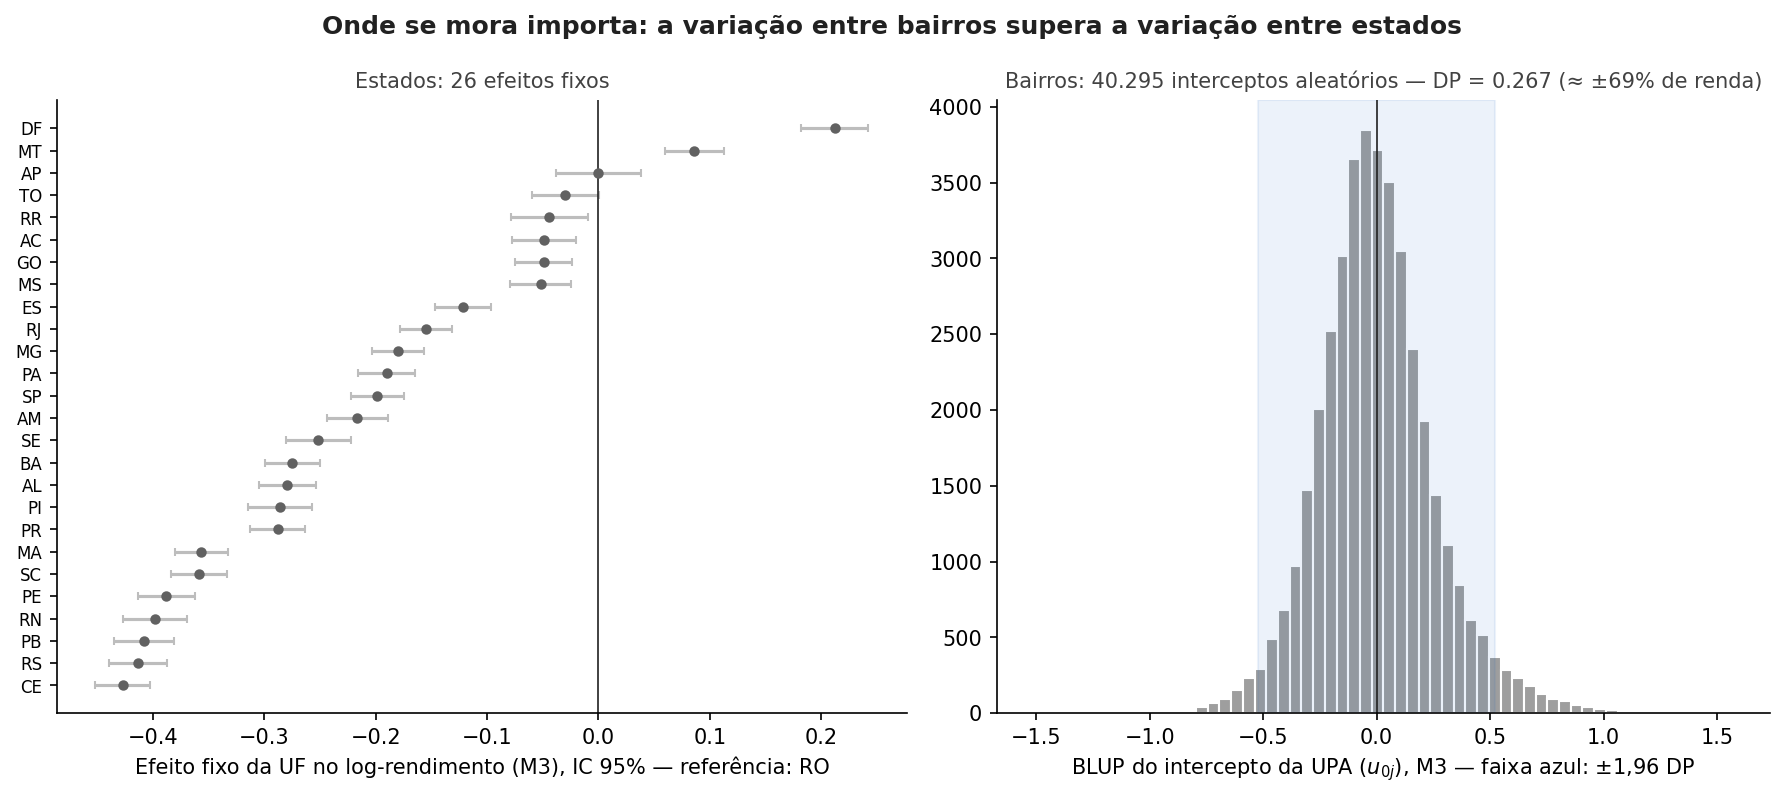
\includegraphics[width=\textwidth]{hlm_efeitos_uf_blup_upa}
  \caption{A variação entre bairros supera a variação entre estados. À esquerda, os
  efeitos fixos de UF do M3 com IC~95\% (referência: primeira UF); à direita, a
  distribuição dos interceptos aleatórios das UPAs ($u_{0j}$, BLUPs do M3).}
  \label{fig:hlm_blups}
\end{figure}
\noindent{Como ler a Figura~\ref{fig:hlm_blups}:} cada ponto à esquerda é um estado;
a largura do histograma à direita é o quanto a renda-base muda de um bairro para outro,
já descontados capital humano, contexto e estado.

\begin{figure}[htbp]
  \centering
  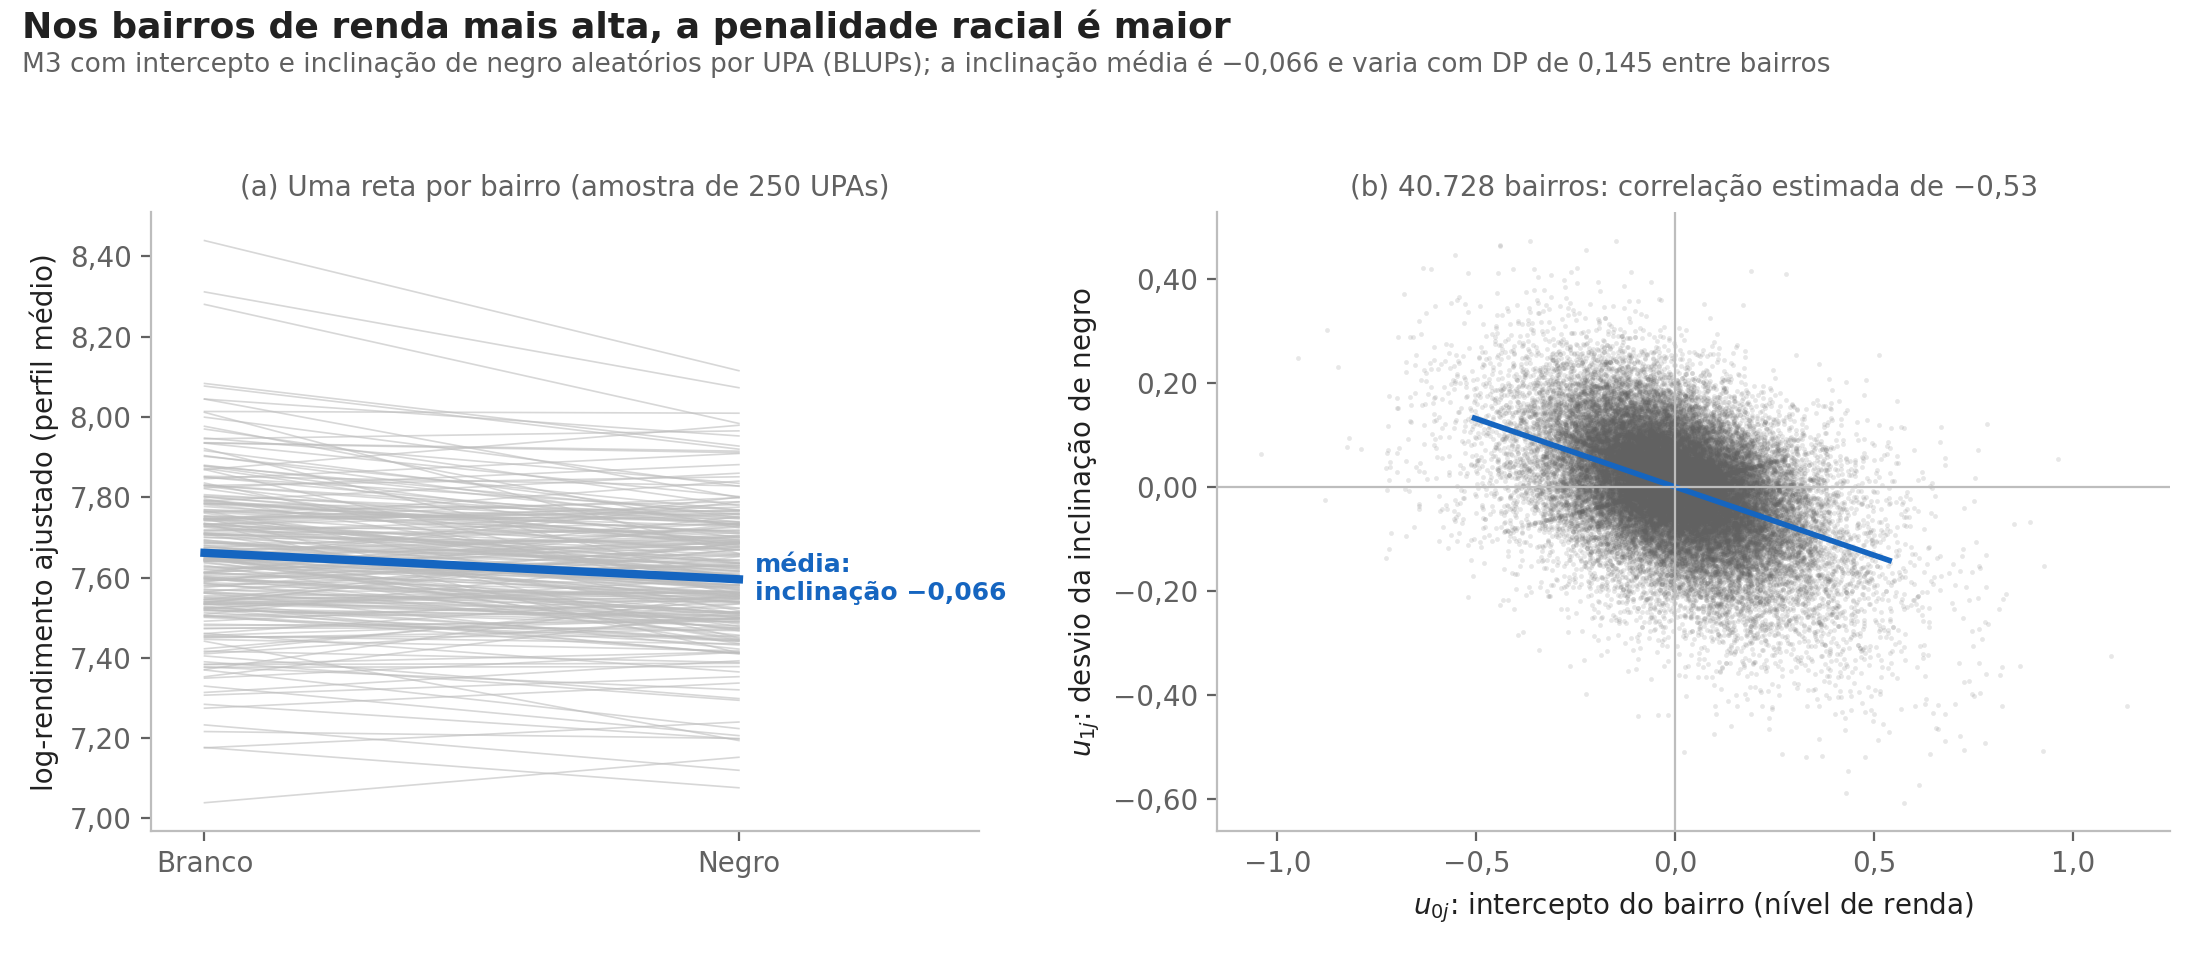
\includegraphics[width=\textwidth]{hlm_rs_retas_upa}
  \caption{Nos bairros de renda mais alta, a penalidade racial é maior. M3 com
  intercepto e inclinação de \texttt{negro} aleatórios por UPA: à esquerda, a reta ajustada
  de cada bairro (amostra de 250 UPAs com brancos e negros) e, em azul, a média; à direita,
  os BLUPs $u_{0j}$ e $u_{1j}$ das 40.728 UPAs, com correlação estimada de
  −0{,}53.}
  \label{fig:hlm_rs}
\end{figure}
\noindent{Como ler a Figura~\ref{fig:hlm_rs}:} à esquerda, a altura de cada reta é a
renda-base do bairro e a inclinação é a penalidade racial dentro dele --- retas que descem
mais são bairros que penalizam mais. À direita, cada ponto é um bairro, e a reta azul resume a
relação: se ela desce, bairros de renda-base maior têm inclinação mais negativa, isto é,
penalizam mais.


\paragraph{A penalidade ao longo da escada educacional.}
O M3 impõe uma única penalidade racial a todos os níveis de escolaridade. Reestimado com o
coeficiente de raça livre em cada nível --- mesma especificação, mesma população ---, ele mostra
que a penalidade condicional diminui da base para o topo da escada: 9{,}6\% entre quem está sem fundamental completo e 1{,}1\% entre quem está com pós-graduação. O teste de razão de verossimilhança contra o M3, que impõe uma penalidade única, rejeita a igualdade entre os níveis (LR $= 3319$, 4~g.l., $p<0{,}001$). Sem controles, o gap mediano é de 14{,}1\% sem fundamental completo e de 26{,}1\% com pós-graduação; a diferença entre o bruto e o condicional, em cada nível, é o que idade, sexo, jornada, bairro e estado explicam ali. A composição também difere: os negros são 67\% de quem está sem fundamental completo e 37\% de quem está com pós-graduação. Como no restante do trabalho, são diferenças condicionais entre pessoas comparáveis, não o efeito de estudar mais.
\begin{figure}[htbp]
  \centering
  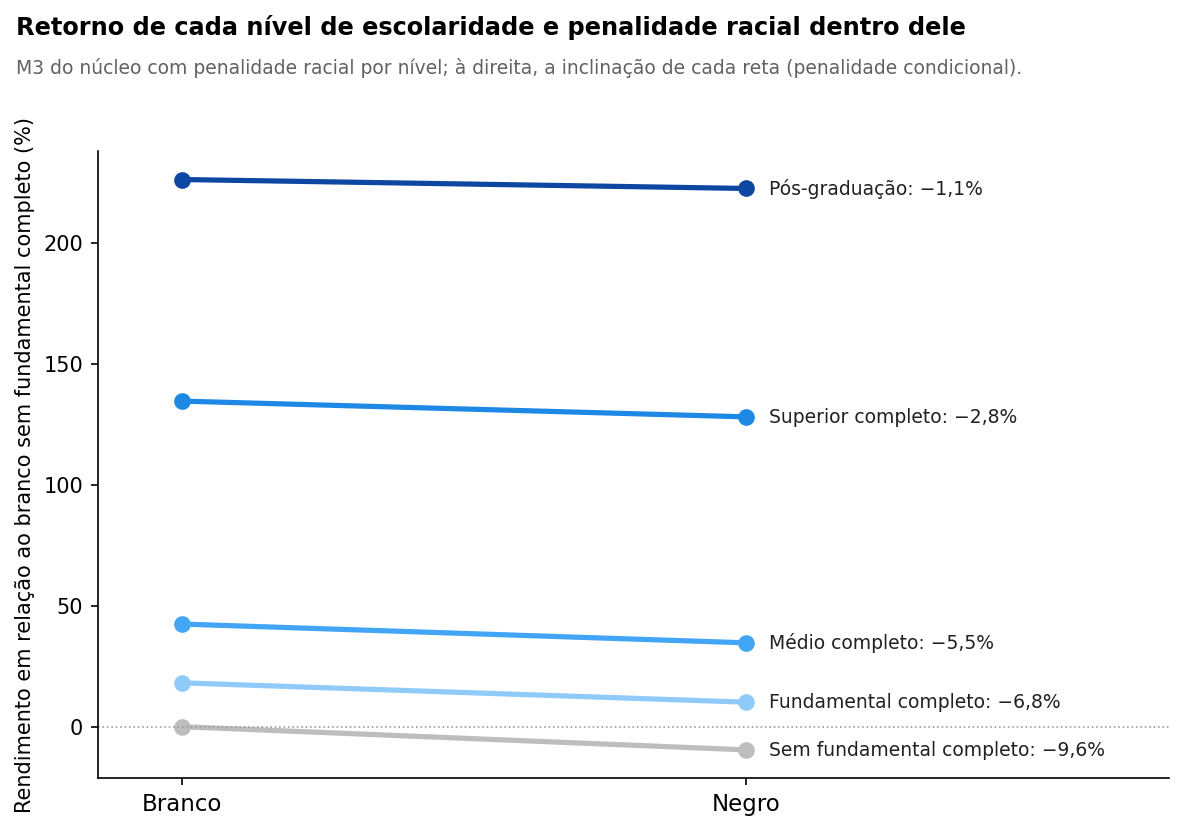
\includegraphics[width=0.9\textwidth]{hlm_negro_por_educ_retas}
  \caption{Retorno de cada nível de escolaridade e penalidade racial dentro dele: M3 do
  núcleo com o coeficiente de raça estimado em cada nível.}
  \label{fig:hlm_negro_educ}
\end{figure}
\noindent{Como ler a Figura~\ref{fig:hlm_negro_educ}:} cada reta é um nível de
escolaridade e vai do trabalhador branco (à esquerda) ao negro (à direita). A altura da reta
é o rendimento do nível em relação ao branco sem fundamental completo; a inclinação é a
penalidade racial dentro do nível, escrita à direita.

\paragraph{O gap verdadeiro está entre dois limites, e nenhum confundidor plausível o anula.}
O coeficiente racial é uma associação condicional: pela fórmula do viés de variável
omitida \cite{angrist2009}, o coeficiente ``curto'' iguala o ``longo'' mais o efeito do
omitido vezes sua relação com a raça. Qualidade da escola, habilidade não observada e
redes de contato correlacionam-se negativamente com ser negro e positivamente com a
renda: omiti-las {superestima} a penalidade --- o que faz do M3 um limite superior
para o efeito de tratamento diferencial condicional a essas características. Na direção
oposta, os controles que são desfechos (ocupação no M4) {subestimam}. O gap líquido
deve ser lido entre esses dois limites. Para anular $\hat\beta^{M3}_{\text{negro}}$ seria
preciso um viés de 98,4\% do coeficiente (Konfound, \citeonline{frank2013}), e o
E-value do modelo de acesso (Tabela~\ref{tab:glmm_glassceil}) exige um confundidor
associado à raça e ao desfecho com razão de risco $\geq 1,5$ --- uma associação
modesta, que sozinha não descarta viés.

\begin{table}[htbp]
\centering
\caption{HLM de dois níveis (indivíduo em UPA) com efeitos fixos de UF --- estratégia {step-up}, PNAD Contínua 2016--2025, população completa ($N = 7.694.080$; 40.728~UPAs; 27~UFs). Coeficientes com erro-padrão do modelo entre parênteses (a correlação intra-UPA já está no efeito aleatório). Estimação por máxima verossimilhança (ML), para os testes LR entre degraus; REML coincide. Com $N$ desta ordem quase todo coeficiente é significante; a inferência relevante está nos intervalos de confiança, não nos asteriscos \cite[cap.~8]{angrist2009}.}
\label{tab:hlm_resultados}
\resizebox{\textwidth}{!}{%
\begin{tabular}{lccccc}
\toprule
\textbf{Variável} & \textbf{M0} & \textbf{M1} & \textbf{M2} & \textbf{M3} & \textbf{M4} \\
\midrule
Intercepto & 7,5778 (0,0028) & 4,8436 (0,0039) & 5,0132 (0,0034) & 5,2269 (0,0078) & 5,4140 (0,0074) \\
\textbf{Raça (negro)} & --- & −0,0669 (0,0005) & −0,0637 (0,0005) & −0,0629 (0,0005) & −0,0579 (0,0005) \\
Sexo feminino & --- & −0,2594 (0,0005) & −0,2590 (0,0005) & −0,2592 (0,0005) & −0,2394 (0,0005) \\
Idade (centrada) & --- & 0,0079 ($<$0,0001) & 0,0078 ($<$0,0001) & 0,0078 ($<$0,0001) & 0,0088 ($<$0,0001) \\
Idade$^2$ & --- & −0,0004 ($<$0,0001) & −0,0004 ($<$0,0001) & −0,0004 ($<$0,0001) & −0,0004 ($<$0,0001) \\
\addlinespace[3pt]
\multicolumn{6}{l}{{Escolaridade (ref.: fundamental incompleto)}} \\
Educ.: fundamental completo & --- & 0,1884 (0,0007) & 0,1880 (0,0007) & 0,1877 (0,0007) & 0,1464 (0,0007) \\
Educ.: médio completo & --- & 0,1965 (0,0007) & 0,1956 (0,0007) & 0,1958 (0,0007) & 0,1013 (0,0007) \\
Educ.: superior completo & --- & 0,5133 (0,0007) & 0,5107 (0,0007) & 0,5112 (0,0007) & 0,2937 (0,0008) \\
Educ.: pós-graduação & --- & 0,3359 (0,0011) & 0,3341 (0,0011) & 0,3350 (0,0011) & 0,2445 (0,0011) \\
\addlinespace[3pt]
\multicolumn{6}{l}{{Inserção}} \\
log(horas) & --- & 0,6536 (0,0006) & 0,6539 (0,0006) & 0,6534 (0,0006) & 0,5801 (0,0006) \\
Urbano & --- & 0,3419 (0,0037) & 0,0927 (0,0032) & 0,0492 (0,0027) & 0,0071 (0,0025) \\
\addlinespace[3pt]
\multicolumn{6}{l}{{Contexto de bairro --- nível 2 (UPA)}} \\
\% negro na UPA ($z$) & --- & --- & −0,1272 (0,0013) & −0,0528 (0,0018) & −0,0576 (0,0017) \\
Desemprego na UPA ($z$) & --- & --- & −0,0183 (0,0012) & −0,0007 (0,0010) & −0,0051 (0,0010) \\
Educ. média na UPA ($z$) & --- & --- & 0,1577 (0,0014) & 0,1694 (0,0013) & 0,1427 (0,0012) \\
\addlinespace[3pt]
\multicolumn{6}{l}{{Ocupação e vínculo (M4; {bad controls})}} \\
Emprego formal & --- & --- & --- & --- & 0,1585 (0,0006) \\
Conta própria & --- & --- & --- & --- & −0,1658 (0,0006) \\
Trab. doméstico & --- & --- & --- & --- & −0,1052 (0,0010) \\
CBO: dirigente & --- & --- & --- & --- & 0,6250 (0,0013) \\
CBO: profissional & --- & --- & --- & --- & 0,5608 (0,0011) \\
CBO: técnico & --- & --- & --- & --- & 0,4001 (0,0010) \\
CBO: administrativo & --- & --- & --- & --- & 0,1771 (0,0010) \\
CBO: serviços & --- & --- & --- & --- & 0,1517 (0,0007) \\
CBO: agropecuária & --- & --- & --- & --- & 0,0844 (0,0010) \\
CBO: operário & --- & --- & --- & --- & 0,1839 (0,0008) \\
CBO: operador & --- & --- & --- & --- & 0,2152 (0,0009) \\
CBO: FFAA & --- & --- & --- & --- & 0,7871 (0,0023) \\
\addlinespace[2pt]
IC 95\% de $\beta_{\text{negro}}$ & --- & [−0,0679; −0,0658] & [−0,0647; −0,0627] & [−0,0639; −0,0619] & [−0,0588; −0,0569] \\
Gap (\%) $= e^{\beta}-1$ & --- & −6,5 & −6,2 & −6,1 & −5,6 \\
Efeitos fixos de UF & não & não & não & sim & sim \\
\addlinespace[2pt] \midrule
\multicolumn{6}{l}{{Componentes de variância e ajuste}} \\
$\hat\tau^2_{\text{UPA}}$ (nível 2) & 0,3018 & 0,1012 & 0,0454 & 0,0297 & 0,0263 \\
$\hat\sigma^2$ (nível 1) & 0,5524 & 0,3619 & 0,3619 & 0,3620 & 0,3237 \\
ICC$_{\text{UPA}}$ & 0,353 & 0,219 & 0,111 & 0,076 & 0,075 \\
$\tau^2$ explicada vs.\ M0 (\%) & --- & 66,5 & 85,0 & 90,1 & 91,3 \\
$-2\,$LL (deviance) & 17.439.754 & 14.160.374 & 14.130.562 & 14.115.850 & 13.255.146 \\
AIC & 17.439.760 & 14.160.418 & 14.130.612 & 14.115.952 & 13.255.272 \\
BIC & 17.439.802 & 14.160.722 & 14.130.959 & 14.116.659 & 13.256.145 \\
LR vs.\ degrau anterior ($\chi^2$, g.l.) & --- & 3.279.380 (19) & 29.811 (3) & 14.712 (26) & 860.704 (12) \\
$p$ do LR & --- & $<0{,}001$ & $<0{,}001$ & $<0{,}001$ & $<0{,}001$ \\
\bottomrule
\end{tabular}}

\noindent\footnotesize{Inclinação aleatória de \texttt{negro} por UPA (M3 + $u_{1j}$):} $\hat\tau^2_{1} = 0,0210$ (DP $= 0,145$ em log-pontos), cov$(u_0,u_1) = −0,0157$; LR $= 26.267$ (2 g.l.), $p<0{,}001$: a penalidade racial varia entre bairros; $\hat\beta_{\text{negro}}$ médio $= −0,0659$.
\normalsize
\par\smallskip\footnotesize Fonte: Resultados originais da pesquisa.
\end{table}


\subsection*{Decomposição do gap por mediação contextual e ocupacional}
A Tabela~\ref{tab:mediacao} resume o resultado central dos modelos HLM: à medida
que se adiciona o bairro (intercepto aleatório e contexto da UPA), o estado e a ocupação,
o gap racial encolhe de 10,5\% (agregado) para 5,6\% (M4); o que resta
no M4 é a penalidade que nenhum atributo observável explica.
\begin{table}[!ht]
\centering
\caption{Decomposição do gap salarial racial por mediação contextual e ocupacional
(HLM de dois níveis, indivíduos em UPA, com efeitos fixos de UF; PNAD Contínua
2016--2025, população completa). Cada linha
acrescenta um bloco de controles ao anterior; à medida que se adiciona contexto e ocupação,
o gap encolhe e a mediação acumulada cresce.}
\label{tab:mediacao}
\resizebox{\textwidth}{!}{%
\begin{tabular}{lrrr}
\toprule
Modelo (controles acumulados) & $\beta_{\text{negro}}$ & Gap (\%) & Mediação acum. (\%) \\
\midrule
Agregado: individual + UF, sem efeito de bairro (OLS) & −0,1104 & −10,5 & --- \\
M1: + intercepto aleatório de bairro (UPA) & −0,0669 & −6,5 & 39,5 \\
M2: + contexto do bairro (UPA) & −0,0637 & −6,2 & 42,3 \\
M3: + efeitos fixos de UF (gap líquido) & −0,0629 & −6,1 & 43,0 \\
M4: + ocupação e formalidade (limite inferior) & −0,0579 & −5,6 & 47,6 \\
\bottomrule
\end{tabular}
}
\par\smallskip
\footnotesize{Como ler:} cada linha adiciona algo à anterior. $\beta_{\text{negro}}$
é a penalidade racial em log-rendimento (mais próximo de zero = menor gap); ``Gap (\%)'' é a
penalidade em \% de renda; ``Mediação acum.''\ é a fração do gap agregado (primeira linha) já
explicada. O salto da primeira para a segunda linha é a mediação pela segregação residencial:
comparar negros e brancos {do mesmo bairro} reduz o gap em 39,5\%. Do modelo agregado
ao M4 o gap cai de 10,5\% para 5,6\%: 47,6\% do gap é mediado por
onde a pessoa mora, o estado e a ocupação que acessa --- e a penalidade de 5,6\% persiste
dentro da mesma ocupação (limite inferior, pois a ocupação é ela própria resultado da barreira de acesso). O agregado inclui efeitos fixos de UF e o M1 e o M2 não (o M3 os reintroduz). Reestimado com UF, na mesma base, o M1 dá $\beta_{\text{negro}} = −0{,}0645$ e uma mediação pelo bairro de 41,6\% (contra 39,5\% na tabela): com o estado mantido no modelo, a mediação pelo bairro é ainda maior --- a leitura da tabela é conservadora. Sem os efeitos fixos de UF, o gap agregado seria de 20,1\% --- a diferença entre estados é, ela própria, parte do diferencial.
\par\smallskip\footnotesize Fonte: Resultados originais da pesquisa.
\end{table}
 A Figura~\ref{fig:hlm_gap} resume a sequência de degraus em barras.

\begin{figure}[htbp]
  \centering
  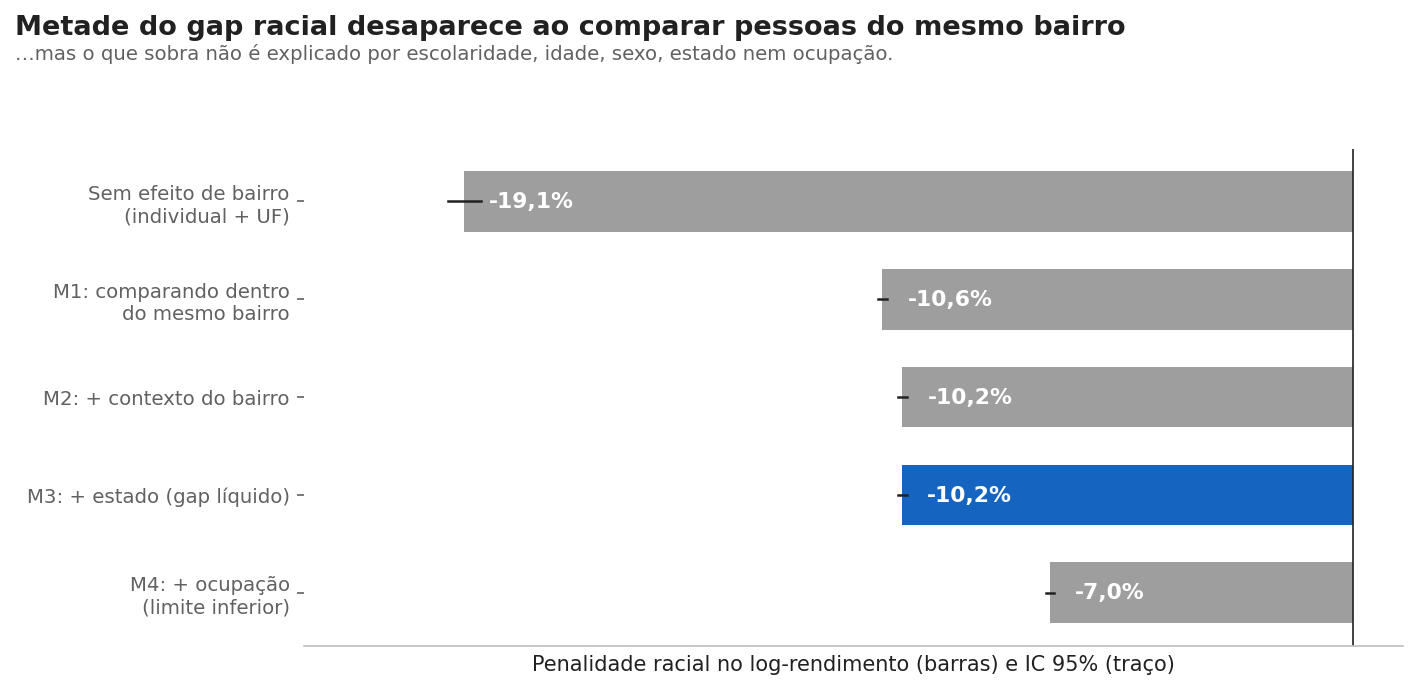
\includegraphics[width=0.92\textwidth]{fig_hlm_gap}
  \caption{Comparar vizinhos reduz o gap em cerca de 40\% --- e o que
  sobra não é explicado por escolaridade, idade, sexo, estado nem ocupação. Barras:
  $\hat\beta_{\text{negro}}$ de cada modelo; traço: IC~95\% (estreito pelo $N$ de milhões);
  rótulo: gap em \% de renda. Em azul, o M3 (gap líquido).}
  \label{fig:hlm_gap}
\end{figure}
\noindent{Como ler a Figura~\ref{fig:hlm_gap}:} cada barra é um modelo da sequência e, de cima para baixo, acrescenta-se um bloco de controles ao anterior. O comprimento da barra é a penalidade racial em log-rendimento e o rótulo dentro dela, a mesma penalidade em \% de renda; o traço fino é o intervalo de confiança de 95\% com erro-padrão agrupado por UPA. Em azul, o M3 --- o gap líquido.

\subsection*{Decomposição de Oaxaca--Blinder: composição {vs.}\ discriminação}
Comparar vizinhos explicou parte do diferencial; resta saber de que é feito o que sobra. De que é feito o gap? Duas explicações rivalizam desde \citeonline{becker1957}, e
elas pedem políticas opostas. Ou negros e brancos chegam ao mercado com características
diferentes e o mercado paga igual por características iguais --- o gap é
{composição}, e a política tem de agir antes do mercado, na escola e na formação.
Ou chegam com as mesmas características e o mercado paga diferente --- o gap é
{preço}, e a política tem de agir dentro dele, na contratação e na fiscalização.
A distinção é empírica, e a decomposição de Oaxaca--Blinder foi construída para fazê-la.

A decomposição de Oaxaca--Blinder separa o gap bruto de log-rendimento
(0,4252 log-pontos, ou 53,0\%) em uma parcela explicada por diferenças de
dotações e uma parcela não explicada (retornos diferenciais --- limite inferior da
discriminação). A Tabela~\ref{tab:oaxaca_blinder} apresenta duas especificações,
porque ocupação e formalidade são {bad controls} \cite{angrist2009}:
são elas próprias resultado da discriminação. Em (A), com os controles do HLM~M3
(capital humano, jornada, contexto de UPA e estado), 17,9\% do gap não é
explicado por características observáveis; em (B), tratando também formalidade e grupo
CBO como dotações, a parcela não explicada cai para 15,4\% --- a
discriminação salarial {dentro} da ocupação. A diferença entre as duas
(2,5 pontos percentuais) é a parcela da discriminação que opera pela
{porta de entrada} das ocupações, e não pelo salário --- exatamente o que o
GLMM de acesso mede adiante. Os erros-padrão vêm de bootstrap em blocos por UPA.

\paragraph{Pressupostos das regressões por grupo.} As duas regressões auxiliares
(brancos e negros) foram submetidas aos testes de Breusch--Pagan e RESET
\cite[cap.~12]{favero2024}. Há heterocedasticidade --- esperada em log-rendimento ---
mas de magnitude modesta: o $R^2$ da regressão auxiliar do Breusch--Pagan é 0,067
(brancos) e 0,066 (negros), e é justamente por isso que os erros-padrão são
agrupados por UPA e a decomposição usa bootstrap em blocos. O RESET rejeita a forma
funcional linear, mas o ganho de $R^2$ ao acrescentar potências do valor predito é de
0,0020 (brancos) e 0,0060 (negros) --- irrelevante para a decomposição. Com $N$
de milhões, ambos os testes rejeitam qualquer hipótese nula pontual; o que importa é a
magnitude, não o $p$-valor \cite{angrist2009}.
\begin{table}[!ht]
\centering
\caption{Decomposição de Oaxaca--Blinder ({twofold}, referência: estrutura de preços
dos brancos) do gap salarial racial em duas especificações. (A)~{Capital humano +
contexto}: escolaridade, idade, sexo, jornada, área urbana, contexto de UPA e efeitos fixos
de UF --- os mesmos controles do HLM~M3; a parcela não explicada é comparável à da literatura.
(B)~{Acesso}: (A) + formalidade e grupo CBO tratados como dotações (os controles do M4) --- a parcela não explicada é a discriminação
{dentro} da ocupação, um limite inferior, pois a segregação ocupacional é ela própria
discriminatória \cite{oaxaca_ransom1999} (ver o GLMM de acesso, Tabela~\ref{tab:glmm_glassceil}).
População completa da PEA com renda positiva ($N = 7.699.278$; 41.459~UPAs).
Erros-padrão entre parênteses: bootstrap em blocos por UPA (500 réplicas).}
\label{tab:oaxaca_blinder}
\resizebox{\textwidth}{!}{%
\begin{tabular}{lcccc}
\toprule
& \multicolumn{2}{c}{(A) Sem ocupação} & \multicolumn{2}{c}{(B) Acesso (com ocupação)} \\
\cmidrule(lr){2-3}\cmidrule(lr){4-5}
Componente & log-pontos (SE) & \% do gap & log-pontos (SE) & \% do gap \\
\midrule
Gap total (branco $-$ negro) & 0,4252 (0,0033) & 100,0 & 0,4252 (0,0032) & 100,0 \\
Dotações (características observáveis) & 0,3491 (0,0033) & 82,1 & 0,3598 (0,0032) & 84,6 \\
Não explicado (retornos / discriminação) & 0,0761 (0,0012) & 17,9 & 0,0654 (0,0011) & 15,4 \\
\bottomrule
\end{tabular}
}
\par\smallskip
\footnotesize{Como ler:} em cada especificação, Dotações $+$ Não explicado $=$ Gap total.
De (A) para (B), parte do ``não explicado'' migra para ``dotações'' porque a ocupação passa a
ser tratada como característica --- é exatamente a parcela da discriminação que opera pela
{porta de entrada}, e não pelo salário.
\par\smallskip\footnotesize Fonte: Resultados originais da pesquisa.
\end{table}
 A Figura~\ref{fig:ob_cascata} apresenta as duas especificações em forma de cascata.

\begin{figure}[htbp]
  \centering
  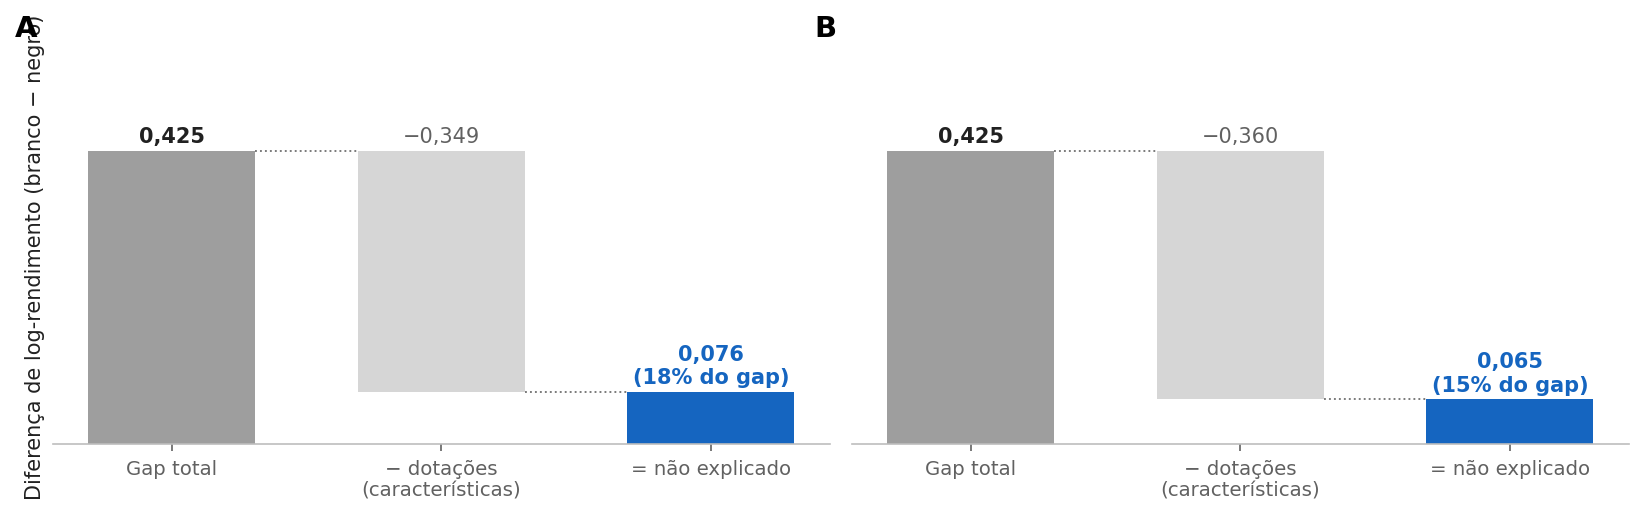
\includegraphics[width=0.95\textwidth]{fig_ob_cascata}
  \caption{Tratar a ocupação como ``característica'' reduz a discriminação medida de
  17,9\% para 15,4\% do gap. Os 2,5 pontos que somem são a parte que
  opera na porta de entrada das ocupações --- medida diretamente pelo modelo de acesso.}
  \label{fig:ob_cascata}
\end{figure}
\noindent{Como ler a Figura~\ref{fig:ob_cascata}:} cada painel é uma cascata lida da esquerda para a direita. A primeira barra é o gap total em log-rendimento; a segunda desconta a parcela atribuída a diferenças de características (dotações); a terceira, em azul, é o que sobra sem explicação. A única diferença entre os painéis é se a ocupação entra ou não como característica.

\subsection*{GLMM logístico: o teto de vidro no acesso}
A decomposição mostrou que parte do diferencial opera na entrada das ocupações; o modelo de acesso mede essa porta diretamente. \label{subsec:glmm_resultados}
Até aqui a pergunta foi quanto um trabalhador negro ganha a menos. Ela pressupõe que
negros e brancos estejam disputando as mesmas vagas. E se a barreira for anterior ao
salário --- se ela estiver em {quais} posições cada um consegue alcançar? É a
pergunta desta subseção, e ela importa porque muda o alvo da política: se a desigualdade
se produz no salário, o remédio é fiscalização de remuneração; se ela se produz no
acesso, nenhuma política salarial a alcança. Três desfechos respondem --- ocupar cargo
qualificado (CBO~1--4), estar no top~20\% e no top~10\% da renda ---, cada um estimado
em quatro degraus próprios, rotulados A1 a A4 para não se confundirem com os do HLM
---aos quais não correspondem um a um---, com intercepto aleatório de UPA e efeitos fixos
de UF.\footnote{\texttt{lme4::glmer} com \texttt{nAGQ = 0} --- os efeitos fixos são estimados
junto com os modos condicionais, aproximação mais rápida que a de Laplace e adequada a $N$
de milhões ---, sobre a população completa.
Os degraus são: A1 individual; A2 $+$ contexto do bairro; A3 $+$ vínculo (formalidade,
setor público, conta própria, doméstico), que é desfecho da própria discriminação e por
isso faz do A3 um limite inferior; A4 $+$ interação \texttt{negro}$\times$credencial. A
Tabela~\ref{tab:glmm_glassceil} traz {odds ratios}, efeitos marginais, ICC e
E-values; a Tabela~\ref{tab:glmm_ajuste}, o ajuste e a classificação.}

\paragraph{O acesso também é ``bairro''.}
A primeira coisa que o modelo mostra é que a lógica territorial do HLM se repete aqui.
Entre \textbf{9\% e 22\% da variância latente do
acesso está entre bairros}\footnote{Correlação intraclasse latente do M1:
0,087 para o cargo qualificado e 0,221 para o top~10\%, com
ICC $= \tau^2/(\tau^2+\pi^2/3)$. O teste de razão de verossimilhança contra o logit sem
efeito aleatório dá LR $=$ 77.940 para o cargo e 80.791 para o top~10\%
(1~g.l., $p<0{,}001$).} --- ou seja, saber apenas em que bairro alguém mora já antecipa
boa parte da chance de essa pessoa chegar a um cargo qualificado, antes de se conhecer
sua escolaridade. E a fração é maior para o top~10\% do que para o cargo qualificado:
quanto mais alto o degrau, mais o endereço pesa.

\paragraph{A porta é mais estreita para negros --- e estreita ainda mais no topo.}
Comparando pessoas do mesmo bairro, com a mesma escolaridade, sexo, idade e estado,
a chance de um trabalhador negro ocupar cargo qualificado é
OR~$=$~0,814\footnote{IC~95\% 0,810--0,818. {Odds ratio} abaixo de~1 é
desvantagem; acima de~1, vantagem.} da chance de um branco --- \textbf{chances ({odds})
19\% menores}. Traduzido para probabilidade, que é a medida a reter
\cite{angrist2009}, são \textbf{2,6 pontos percentuais} a menos de chegar
lá. E a desvantagem cresce à medida que se sobe na renda: para chegar ao top~10\% ---
que já não é o acesso a uma ocupação, mas a uma faixa de rendimento --- o OR cai para
0,761, \textbf{chances 24\% menores}. Não é o mesmo fenômeno do
salário visto de outro ângulo --- é uma barreira que age antes, na distribuição das
posições, e que nenhuma política de remuneração igual alcançaria.

Em síntese, a desigualdade racial no mercado de trabalho brasileiro não começa
só no contracheque: começa também na porta.

\paragraph{Vínculo e credencial não desfazem a barreira.}
Duas explicações alternativas se apresentam naturalmente, e o modelo testa as duas. A
primeira é a informalidade: a barreira seria um artefato de negros estarem mais em
vínculos precários. Descontar o vínculo (A3) praticamente não move o OR do cargo
qualificado (0,791) nem o do top~10\% (0,740), de modo que não é
isso. A segunda é o diploma: bastaria credenciar-se. A interação
\texttt{negro}$\times$credencial do A4 é de 1,042 para o superior completo e
0,947 para a pós-graduação --- o superior completo atenua levemente a barreira, mas a pós-graduação volta a agravá-la ---, e o OR combinado de um
trabalhador negro com superior completo ainda é 0,818. A credencial não
neutraliza a barreira. A Figura~\ref{fig:glmm_or} reúne as razões
de chance dos três desfechos e dos modelos de cada um.

\paragraph{Quão forte teria de ser um confundidor omitido.}
O modelo separa bem quem acessa de quem não acessa\footnote{AUC de 0,878 com
efeitos aleatórios e 0,870 só com efeitos fixos, para o cargo qualificado;
no {cutoff} de Youden (0,30), sensibilidade 0,79 e
especificidade 0,79. O teste de Hosmer--Lemeshow rejeita a calibração
perfeita em todos os degraus --- inevitável com $N$ de milhões \cite{angrist2009} ---,
mas a estatística cai 69\% no top~20\% e 54\% no top~10\%, embora suba no cargo qualificado ao se acrescentar o vínculo (A3).}, mas a
pergunta que interessa não é essa: é se a desvantagem poderia ser obra de algo que o
modelo não viu. O E-value responde quanto um confundidor omitido teria de ser forte para
anular o resultado, e aqui ele vale \textbf{1,5}: seria preciso uma
característica não medida associada tanto a ser negro quanto a ocupar cargo qualificado
com razão de risco de pelo menos 1,5 em ambas as pontas (com o desfecho comum, a
razão de chances é convertida em razão de risco pela raiz quadrada). É uma associação
modesta --- a escolaridade, sozinha, tem efeito muito maior sobre o acesso ---, e por isso o
E-value não basta para descartar viés: o que sustenta o resultado é ele sobreviver ao
contexto de bairro e ao teste de Konfound do modelo de renda. Por fim,
o logit com efeitos fixos de UF e erro-padrão agrupado por UPA (última coluna da
Tabela~\ref{tab:glmm_glassceil}) reproduz os OR a partir do A2 (cargo qualificado: 0,796 contra 0,814); no A1, sem o contexto do bairro, dá 0,728 contra 0,805, porque sem o intercepto de UPA o contexto omitido é absorvido pelo coeficiente racial. Com o contexto do bairro no modelo, a conclusão não depende da hipótese de efeitos aleatórios.

\begin{figure}[htbp]
  \centering
  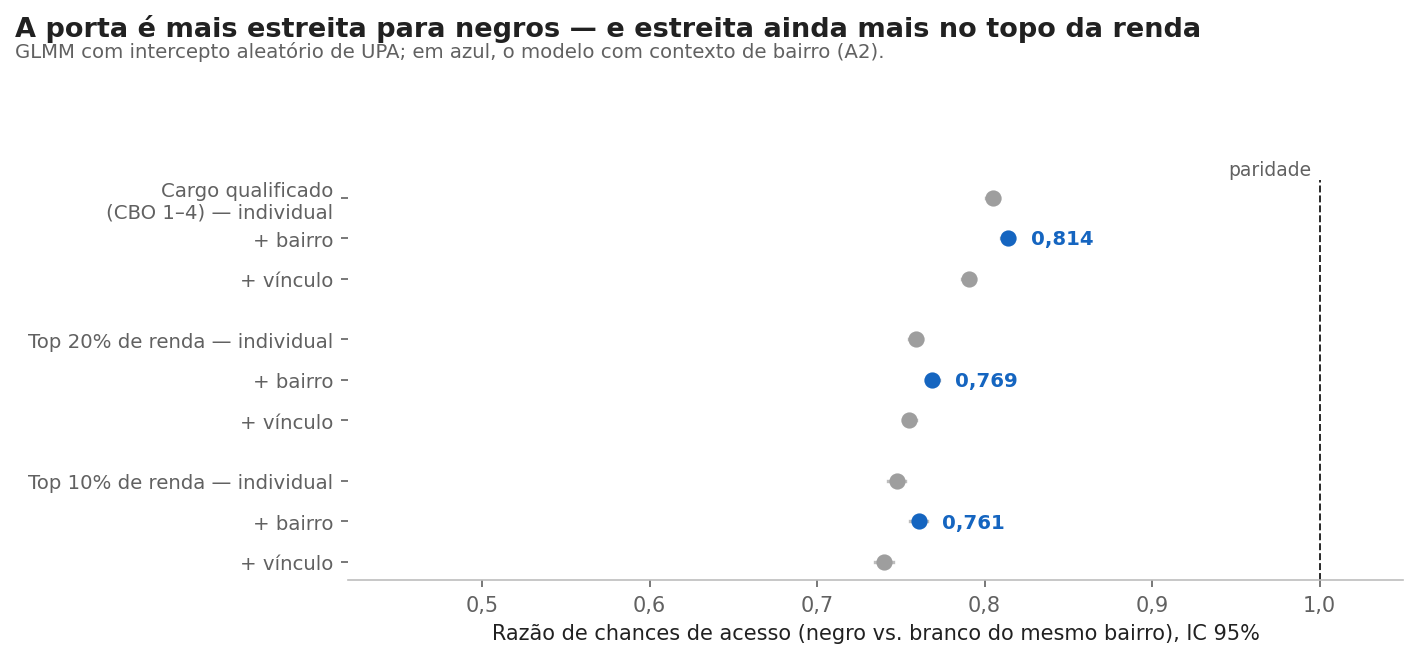
\includegraphics[width=0.95\textwidth]{fig_glmm_or}
  \caption{A porta é mais estreita para trabalhadores negros --- e estreita ainda mais no
  topo da renda. Razão de chances de acesso (negro {vs.}\ branco do mesmo bairro) com
  IC~95\%, por desfecho e degrau; em azul, o modelo com contexto de bairro (A2).}
  \label{fig:glmm_or}
\end{figure}
\noindent{Como ler a Figura~\ref{fig:glmm_or}:} cada ponto é uma razão de chances e a linha horizontal, seu intervalo de confiança de 95\%; a linha tracejada em~1 marca a paridade, de modo que quanto mais à esquerda, maior a desvantagem. Os blocos são os três desfechos e, dentro de cada um, os modelos; em azul, o A2, que compara pessoas do mesmo bairro.

\begin{table}[!ht]
\centering
\caption{GLMM logístico (lme4::\texttt{glmer}, intercepto aleatório de UPA e efeitos fixos de UF) --- teto de vidro ocupacional e salarial. {Odds ratio} do coeficiente \texttt{negro} com IC~95\%, efeito marginal médio (AME: diferença média de probabilidade predita, em pontos percentuais), ICC da UPA $=\tau^2/(\tau^2+\pi^2/3)$ e E-value \cite{vanderweele2017}. Coluna final: OR do logit com efeitos fixos de UF e erro-padrão agrupado por UPA (robustez). População completa da PEA com renda positiva ($N = 7.699.273$; 41.454~UPAs). A3 acrescenta o vínculo (formalidade, setor público, conta própria, doméstico), que é desfecho da própria discriminação: limite inferior. Todos os OR com $p<0{,}001$; com $N$ desta ordem, a inferência relevante está nos IC e nos E-values.}
\label{tab:glmm_glassceil}
\resizebox{\textwidth}{!}{%
\begin{tabular}{llcccccc}
\toprule
Desfecho & Modelo & OR (IC 95\%) & AME (p.p.) & ICC$_{\text{UPA}}$ & E-value & E-value (IC) & OR logit-FE \\
\midrule
Cargo qualificado (CBO 1--4) & A1 individual + UF & 0,805 [0,801; 0,809] & −2,75 & 0,087 & 1,47 & 1,47 & 0,728 \\
 & A2 + contexto do bairro & 0,814 [0,810; 0,818] & −2,60 & 0,054 & 1,46 & 1,45 & 0,796 \\
 & A3 + vínculo (limite inf.) & 0,791 [0,787; 0,794] & −2,66 & 0,054 & 1,50 & 1,49 & 0,796 \\
 & A4 + negro$\times$credencial & 0,785 [0,781; 0,789] & −2,66 & 0,054 & 1,51 & 1,50 & 0,792 \\
\midrule
Top 20\% de renda & A1 individual + UF & 0,759 [0,755; 0,763] & −2,91 & 0,159 & 1,56 & 1,55 & 0,638 \\
 & A2 + contexto do bairro & 0,769 [0,765; 0,773] & −2,77 & 0,083 & 1,54 & 1,53 & 0,756 \\
 & A3 + vínculo (limite inf.) & 0,755 [0,751; 0,759] & −2,80 & 0,084 & 1,57 & 1,56 & 0,756 \\
 & A4 + negro$\times$credencial & 0,719 [0,714; 0,723] & −2,79 & 0,084 & 1,64 & 1,63 & 0,713 \\
\midrule
Top 10\% de renda & A1 individual + UF & 0,748 [0,743; 0,753] & −1,77 & 0,221 & 2,01 & 1,99 & 0,577 \\
 & A2 + contexto do bairro & 0,761 [0,756; 0,766] & −1,66 & 0,116 & 1,96 & 1,94 & 0,739 \\
 & A3 + vínculo (limite inf.) & 0,740 [0,735; 0,745] & −1,73 & 0,117 & 2,04 & 2,02 & 0,739 \\
 & A4 + negro$\times$credencial & 0,668 [0,662; 0,674] & −1,71 & 0,117 & 2,36 & 2,33 & 0,659 \\
\bottomrule
\end{tabular}}
\par\smallskip
\footnotesize{Como ler:} OR $<1$ = menor chance de acesso para trabalhadores negros do que para brancos de mesmo perfil {e do mesmo bairro}; quanto mais perto de zero, maior a barreira. O E-value é a força mínima de associação (razão de risco) que um confundidor não observado precisaria ter com a raça {e} com o desfecho para anular o OR; o E-value (IC) faz o mesmo para o limite do intervalo. A coluna logit-FE mostra que a conclusão não depende da hipótese de efeitos aleatórios.
\par\smallskip\footnotesize Fonte: Resultados originais da pesquisa.
\end{table}

\begin{table}[!ht]
\centering
\caption{GLMM logístico --- ajuste e desempenho de classificação por degrau. LR vs.\ pooled: teste de razão de verossimilhança do A2 contra o logit sem efeito aleatório (fronteira, $p/2$); AUC com efeitos aleatórios (ajuste na amostra) e só com efeitos fixos; {cutoff} de Youden (maximiza sensibilidade $+$ especificidade) com as taxas correspondentes; Hosmer--Lemeshow em 10 decis. Modelos A1--A4 como na Tabela~\ref{tab:glmm_glassceil}. Com $N = 7{,}7$~milhões qualquer desvio de calibração é ``significativo'' --- o $\chi^2$ deve ser lido como magnitude relativa entre degraus, não como teste (MHE, cap.~8).}
\label{tab:glmm_ajuste}
\resizebox{\textwidth}{!}{%
\begin{tabular}{llcccccccc}
\toprule
Desfecho & Modelo & $-2\,$LL & AIC & LR vs.\ pooled & AUC (RE) & AUC (FE) & Cutoff & Sens./Espec. & HL $\chi^2$ \\
\midrule
Cargo qualificado (CBO 1--4) & A1 & 6.102.483 & 6.102.575 & --- & 0,879 & 0,864 & 0,30 & 0,79/0,79 & 2.760 \\
 & A2 & 6.088.976 & 6.089.074 & 77.940 & 0,878 & 0,870 & 0,30 & 0,79/0,79 & 2.796 \\
 & A3 & 5.457.265 & 5.457.373 & --- & 0,906 & 0,900 & 0,31 & 0,83/0,82 & 7.982 \\
 & A4 & 5.457.207 & 5.457.319 & --- & 0,906 & 0,900 & 0,31 & 0,83/0,82 & 7.881 \\
\midrule
Top 20\% de renda & A1 & 5.271.208 & 5.271.300 & --- & 0,872 & 0,845 & 0,19 & 0,79/0,79 & 9.078 \\
 & A2 & 5.251.296 & 5.251.394 & 108.283 & 0,872 & 0,859 & 0,19 & 0,79/0,79 & 9.584 \\
 & A3 & 4.967.208 & 4.967.316 & --- & 0,886 & 0,875 & 0,19 & 0,81/0,80 & 2.956 \\
 & A4 & 4.966.299 & 4.966.411 & --- & 0,886 & 0,875 & 0,19 & 0,81/0,80 & 2.630 \\
\midrule
Top 10\% de renda & A1 & 3.276.689 & 3.276.781 & --- & 0,901 & 0,868 & 0,09 & 0,83/0,81 & 6.085 \\
 & A2 & 3.258.340 & 3.258.438 & 80.791 & 0,900 & 0,886 & 0,09 & 0,83/0,81 & 6.176 \\
 & A3 & 3.075.653 & 3.075.761 & --- & 0,913 & 0,900 & 0,10 & 0,83/0,83 & 2.836 \\
 & A4 & 3.074.632 & 3.074.744 & --- & 0,913 & 0,900 & 0,09 & 0,85/0,82 & 2.472 \\
\bottomrule
\end{tabular}}
\par\smallskip\footnotesize Fonte: Resultados originais da pesquisa.
\end{table}


\subsection*{Regressão Quantílica e RIF-OB: teto de vidro e {sticky floor}}
Passada a porta, resta a escada: a penalidade é a mesma para quem ganha pouco e para quem ganha muito? \label{subsec:qr_rif}
A penalidade racial é a mesma em toda a distribuição de renda? Nada obriga que seja,
e as duas possibilidades apontam para lugares diferentes. Se ela crescer rumo ao topo, o
problema é um teto de vidro: quanto mais alto se sobe, mais a cor pesa, e o alvo da
política são as posições de comando. Se for maior na base, o problema é um piso
pegajoso, e concentrar esforços nas elites profissionais erra o alvo por inteiro. Os
resultados a seguir mostram que as duas leituras estão corretas --- porque respondem a
perguntas diferentes, e a subseção termina explicando por que não se contradizem.

A regressão quantílica estima o gap em cada ponto da distribuição de renda; a
RIF-OB separa, por quantil, dotação e retorno. A Tabela~\ref{tab:qr_melhorias}
mostra a penalidade {condicional} crescendo rumo ao topo (teto de vidro entre
pessoas de mesmo perfil); a
Tabela~\ref{tab:rif_ob} revela o padrão complementar: o componente de retorno
(discriminação proporcional) é maior na base e {decresce} rumo ao topo
({sticky floor}). {Como ler:} na Tabela~\ref{tab:rif_ob}, Dotações $+$
Retornos $=100\%$ do gap RIF --- a coluna ao lado do gap observado ---,
e a coluna Retornos cai de $26{,}5\%$ (q10) a $8{,}9\%$ (q90):
a parcela não explicada pesa mais na base. Como a RIF usa os controles da
Oaxaca--Blinder {sem} ocupação, sua parcela de retornos na mediana
($20{,}6\%$) se compara aos $17{,}9\%$ da especificação (A)
da Tabela~\ref{tab:oaxaca_blinder}, e não aos $15{,}4\%$ da (B), que trata a
ocupação como característica. O q25 pede cautela: ele cai sobre o salário mínimo,
onde muitos trabalhadores têm exatamente a mesma renda. Num ponto de massa assim a
densidade que a RIF usa não é bem definida e depende da largura de banda do
{kernel}; por isso, no q25, o gap que a RIF decompõe fica bem abaixo do
observado. As parcelas de dotações e retornos, que são razões, não dependem dessa
escolha --- a densidade escala as duas pelo mesmo fator ---, e o padrão do q10 ao q90
também não.

\paragraph{Por sexo.} As colunas por sexo da Tabela~\ref{tab:qr_melhorias} mostram que o padrão não é o mesmo para todos: entre homens, a penalidade cresce de 3,9\% (q10) para 9,0\% (q90); entre mulheres, a penalidade é maior nas duas pontas --- 4,9\% no q10, 4,3\% na mediana e 7,3\% no q90 ---, de modo que ao teto de vidro se soma um piso pegajoso {condicional}.

\paragraph{Por que os dois padrões não se contradizem.} A regressão quantílica
estima quantis {condicionais}: $\hat\beta(\tau)$ compara negros e brancos na
mesma posição {dentro} da distribuição de pessoas com o mesmo perfil observável.
O crescimento de $|\hat\beta(\tau)|$ ao longo de $\tau$ significa que a dispersão
condicional do rendimento é maior entre brancos --- {fanning out} na linguagem de
\citeonline{angrist2009} ---, e não que ``os negros do topo sofrem mais'': quantis não
seguem indivíduos, e a leitura em termos de pessoas exigiria invariância de posto, que
não se testa aqui. A RIF-OB, ao contrário, decompõe quantis {incondicionais} da
distribuição de renda \cite{firpo2018}: responde ``de que é feito o gap no q10 da renda
do país''. Como a composição observável concentra negros na base, a parcela de retornos
é maior ali; e como há mais dispersão condicional no topo, o coeficiente condicional
cresce com $\tau$. Os dois resultados são complementares --- um é sobre o {preço}
pago a características, o outro sobre a {distribuição} de características.
\begin{table}[H]
\centering
\caption{Regressão quantílica: coeficiente $\hat{\beta}_{\text{negro}}$ por quantil e sexo.
         Gap~(\%) $= (e^{\hat{\beta}}-1)\times 100$.
         M3: controles individuais + contexto UPA + UF efeito fixo. População completa.
         Entre parênteses (coluna Global): erro-padrão por bootstrap em blocos por UPA.
         $^{***}p<0{,}001$ em todos os quantis e grupos.}
\label{tab:qr_melhorias}
\small
\begin{tabular}{lrrrrrr}
\toprule
& \multicolumn{2}{c}{Global} & \multicolumn{2}{c}{Homens} & \multicolumn{2}{c}{Mulheres} \\
\cmidrule(lr){2-3}\cmidrule(lr){4-5}\cmidrule(lr){6-7}
Quantil & $\hat{\beta}$ (SE) & Gap~(\%) & $\hat{\beta}$ & Gap~(\%) & $\hat{\beta}$ & Gap~(\%) \\
\midrule
$\tau=0{,}10$ & $-0{,}0437$ (0{,}0014) & $-4{,}3\%$ & $-0{,}0402$ & $-3{,}9\%$ & $-0{,}0502$ & $-4{,}9\%$ \\
$\tau=0{,}25$ & $-0{,}0435$ (0{,}0009) & $-4{,}3\%$ & $-0{,}0424$ & $-4{,}2\%$ & $-0{,}0454$ & $-4{,}4\%$ \\
$\tau=0{,}50$ & $-0{,}0504$ (0{,}0008) & $-4{,}9\%$ & $-0{,}0537$ & $-5{,}2\%$ & $-0{,}0444$ & $-4{,}3\%$ \\
$\tau=0{,}75$ & $-0{,}0670$ (0{,}0010) & $-6{,}5\%$ & $-0{,}0723$ & $-7{,}0\%$ & $-0{,}0583$ & $-5{,}7\%$ \\
$\tau=0{,}90$ & $-0{,}0875$ (0{,}0014) & $-8{,}4\%$ & $-0{,}0940$ & $-9{,}0\%$ & $-0{,}0757$ & $-7{,}3\%$ \\
$\tau=0{,}95$ & $-0{,}1035$ (0{,}0020) & $-9{,}8\%$ & $-0{,}1092$ & $-10{,}3\%$ & $-0{,}0920$ & $-8{,}8\%$ \\
\midrule
\textbf{Δ (q90−q10)} & $\mathbf{-0{,}0439\text{ log-pt}}^{***}$ (0{,}0017) & \multicolumn{2}{c}{$Z = -25{,}87$} & \multicolumn{2}{c}{$p < 0{,}001$} \\
\bottomrule
\end{tabular}
\note{Teste de heterogeneidade quantílica (Koenker-Bassett style):
      $H_0$: $\hat{\beta}(q)$ constante para todo $q$.
      SE por bootstrap em blocos por UPA, ``$m$ de $n$'' ($B=200$; $m=1.243$ das $41.459$ UPAs por réplica;
      SE escalado por $\sqrt{m/G}$, Bickel \& Sakov, 2008). Sem a escala (conservador): $Z=-4{,}48$, $p < 0{,}001$.}
\par\smallskip\footnotesize Fonte: Resultados originais da pesquisa.
\end{table}

\begin{table}[!ht]
\centering
\caption{Decomposição RIF-OB \cite{firpo2018} do gap salarial racial
por quantil incondicional, em formato {two-fold} (referência: estrutura de preços
dos brancos). Mesmos controles da decomposição de Oaxaca--Blinder sem ocupação (escolaridade,
idade, sexo, jornada, área urbana, ano e contexto do bairro), mais efeitos fixos de UF; a ocupação {não} entra.
Dotações: diferença de características observáveis. Retornos: parcela não explicada, que
inclui a discriminação e o que não foi observado. Dotações + Retornos
$=100\%$ {do gap RIF} --- que é o gap decomposto pelo
método e difere do gap observado da segunda coluna; as porcentagens
são fração daquele, não deste. Padrão {sticky floor}: a parcela de retornos
é maior na base e decresce rumo ao topo. PNAD Contínua 2016--2025,
população completa. Entre parênteses: erro-padrão por bootstrap em blocos por UPA.}
\label{tab:rif_ob}
\begin{tabular}{lrrrrr}
\toprule
Quantil & Gap obs. (SE) & Gap RIF & Dotações (\%) & Retornos (\%) & $N$ \\
\midrule
q10 & 0,569 (0,005) & 0,536 & 73,5 (0,7) & 26,5 (0,6) & 7.699.278 \\
q25 & 0,223 (0,005) & 0,130 & 77,7 (1,0) & 22,3 (0,6) & 7.699.278 \\
q50 & 0,375 (0,003) & 0,427 & 79,4 (0,7) & 20,6 (0,3) & 7.699.278 \\
q75 & 0,448 (0,004) & 0,462 & 83,1 (1,3) & 16,9 (0,4) & 7.699.278 \\
q90 & 0,564 (0,007) & 0,573 & 91,1 (1,6) & 8,9 (0,5) & 7.699.278 \\
\bottomrule
\end{tabular}
\par\smallskip\footnotesize Fonte: Resultados originais da pesquisa.
\end{table}
 A Figura~\ref{fig:qr_rif} põe os dois ângulos lado a lado.

\begin{figure}[htbp]
  \centering
  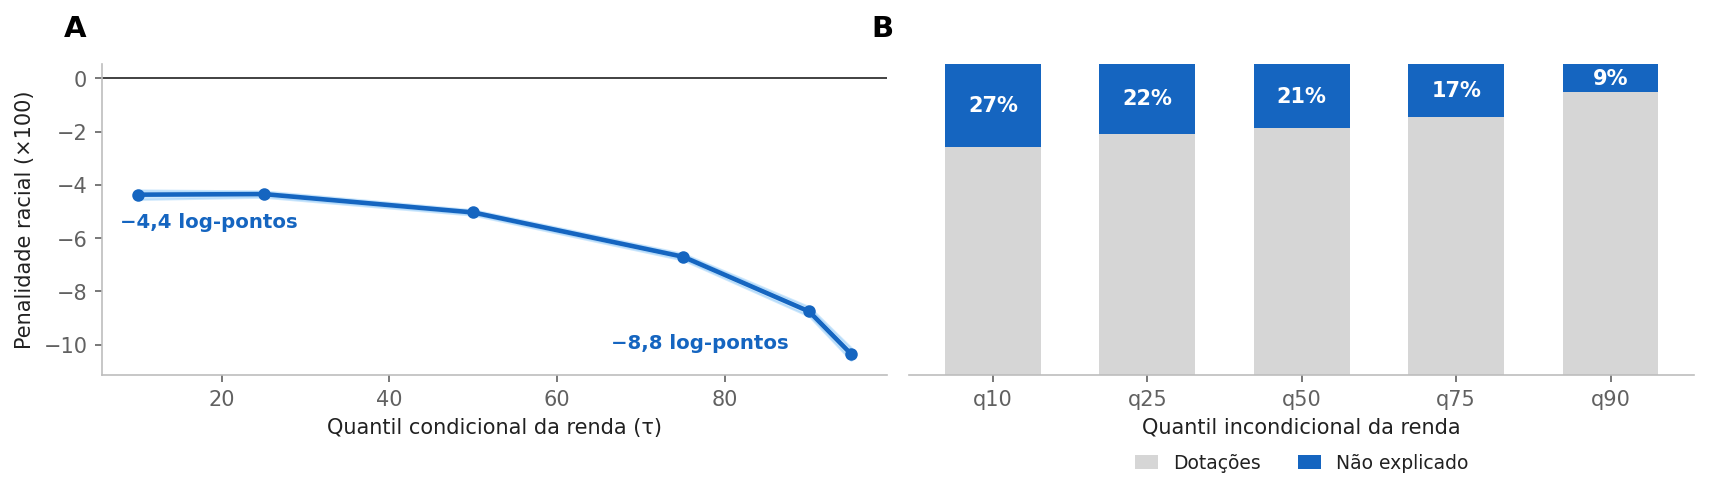
\includegraphics[width=0.98\textwidth]{fig_qr_rif}
  \caption{Teto de vidro entre pares, piso pegajoso na renda do país: duas perguntas,
  dois padrões. À
  esquerda, a penalidade em quantis {condicionais} cresce rumo ao topo (faixa: IC~95\%
  por bootstrap em blocos de UPA); à direita, a parcela não explicada dos quantis
  {incondicionais} da renda é maior na base.}
  \label{fig:qr_rif}
\end{figure}
\noindent{Como ler a Figura~\ref{fig:qr_rif}:} à esquerda, cada ponto é a penalidade racial estimada num quantil {condicional} $\tau$ (eixo vertical em log-pontos $\times100$), e a faixa é o intervalo de 95\% por bootstrap em blocos de UPA. À direita, cada barra é um quantil {incondicional} da renda e soma 100\%: a parte azul é a parcela não explicada, com o valor escrito dentro.

\subsection*{Interseccionalidade: raça e gênero no acesso e no topo}
Até aqui, raça foi tratada como um eixo só; a última etapa pergunta quem está na interseção. \label{subsec:interseccional}

Raça e gênero simplesmente se somam? Todos os modelos até aqui responderam que sim,
por construção: tratadas como penalidades aditivas, a desvantagem de ser negra {e}
mulher seria a de ser negro mais a de ser mulher. \citeonline{crenshaw1989} desconfia
dessa aritmética, e a desconfiança é testável --- basta trocar os dois indicadores
separados por um único fator de quatro grupos e deixar que os dados digam se a soma
fecha.\footnote{GLMM de acesso reespecificado com \texttt{grupo\_rg} (homem branco como
referência, mulher branca, homem negro, mulher negra) e a interação
\texttt{negro$\times$sexo\_fem}, em três desfechos: ocupação qualificada (CBO~1--4),
renda no top~20\% e no top~10\%.} A Tabela~\ref{tab:interseccional} traz a decomposição de Oaxaca--Blinder dos quatro grupos contra o homem branco, e a Figura~\ref{fig:interseccional}, as razões de chance nos três desfechos.

\begin{table}[!ht]
\centering
\caption{Decomposição interseccional (raça $\times$ gênero) do gap de rendimento
{vs.}\ o Homem Branco (grupo de referência). Dotações: parcela explicada por
características observáveis; Retornos: parcela não explicada (discriminação). Gap (log):
a mesma desvantagem em log-pontos, a escala em que os efeitos de raça e de gênero se somam
\cite{crenshaw1989}. PNAD Contínua, população completa
($N$ do grupo de referência --- homens brancos --- na última linha da nota). Entre
parênteses: erro-padrão por bootstrap em blocos por UPA.}
\label{tab:interseccional}
\resizebox{\textwidth}{!}{%
\begin{tabular}{lrrrrr}
\toprule
Grupo & Gap vs HB (\%) & Gap (log) & Dotações (\%) & Retornos (\%) & $N$ do grupo \\
\midrule
Mulher Branca & 19,9 (0,2) & 0,182 & −97,0 (1,8) & 197,0 (1,8) & 1.429.355 \\
Homem Negro & 56,4 (0,5) & 0,447 & 77,2 (0,3) & 22,8 (0,3) & 2.662.039 \\
Mulher Negra & 80,7 (0,6) & 0,592 & 27,4 (0,4) & 72,6 (0,4) & 1.765.796 \\
\bottomrule
\end{tabular}
}
\par\smallskip
\footnotesize{Como ler:} ``Gap vs HB'' é a desvantagem de renda de cada grupo
{vs.}\ o Homem Branco; Dotações $+$ Retornos $=100\%$ do gap. A Mulher Negra tem o
maior gap. Em log-pontos, o gap da Mulher Negra (0,592) fica abaixo da soma dos gaps da Mulher Branca e do Homem Negro (0,629): as desvantagens de raça e de gênero se acumulam sem se multiplicar --- a interação é sub-aditiva, como no modelo de acesso. Somar os percentuais daria a impressão contrária, porque a escala percentual é convexa. O sinal negativo das dotações da Mulher
Branca indica que suas características observáveis {superam} as do homem branco: todo
o gap vem de retornos diferenciais. Grupo de referência: 1.842.088 homens brancos.
\par\smallskip\footnotesize Fonte: Resultados originais da pesquisa.
\end{table}


\begin{figure}[htbp]
  \centering
  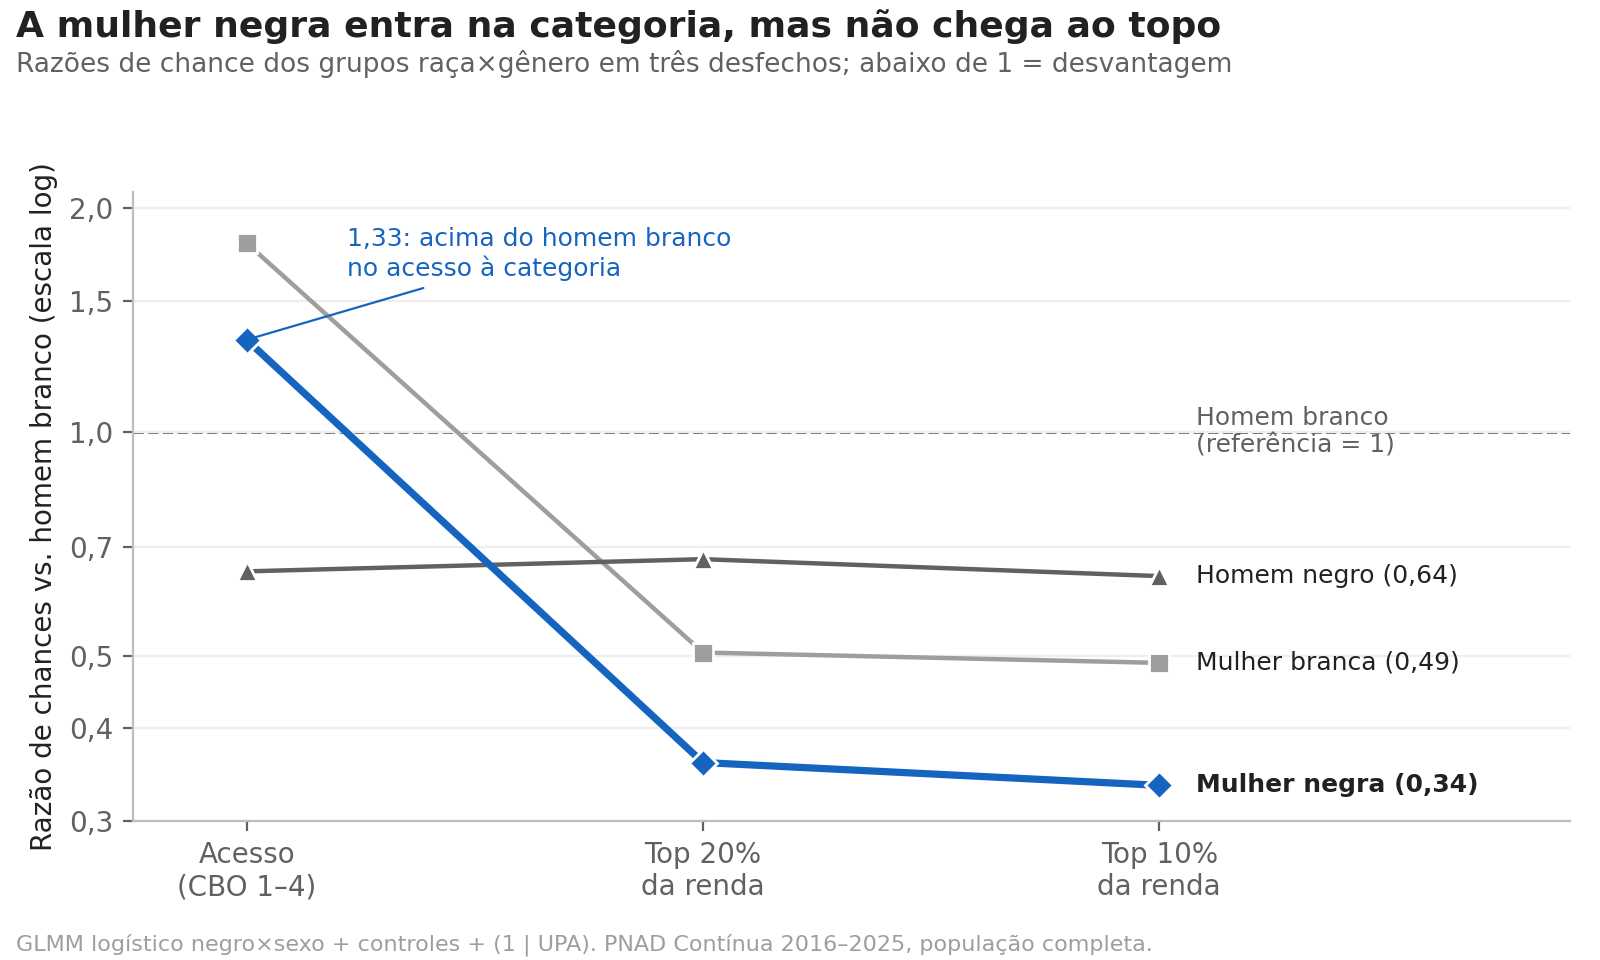
\includegraphics[width=0.82\textwidth]{grupo_rg_interseccional}
  \caption{A vantagem aparente da mulher negra no acesso é de composição: razões de chance dos quatro grupos raça$\times$gênero {vs.}~homem
  branco, em três desfechos. Na categoria agregada ela aparece acima da referência,
  mas por composição: entra pelas ocupações feminizadas e é a mais distante do homem
  branco entre os dirigentes e no topo da renda.}
  \label{fig:interseccional}
\end{figure}
\noindent{Como ler a Figura~\ref{fig:interseccional}:} cada série é um grupo raça$\times$gênero e cada ponto, a razão de chances contra o homem branco, cuja referência é a linha tracejada em 1; abaixo dela, o grupo tem menos chance que ele. À esquerda, siga a série azul (mulher negra): ela aparece acima da referência na categoria agregada e termina como o grupo mais distante da referência no topo da renda. À direita, a mesma comparação por grande grupo da CBO mostra de onde vem a aparente vantagem: das ocupações feminizadas, não do comando.

\paragraph{Na entrada, a vantagem da mulher negra é de ocupações feminizadas.}
No acesso à ocupação qualificada (CBO~1--4) a mulher negra tem OR~$=1,31$,
mais chance do que o homem branco de referência, e o grupo mais penalizado na entrada
é o \textbf{homem negro} (OR~$=0,76$). O agregado, porém, junta portas
muito diferentes, e estimar o mesmo modelo para cada grande grupo da CBO muda o
quadro. A aparente vantagem da mulher negra no acesso a cargos CBO~1--4 é composição: vem do apoio administrativo (OR 1,96) e das profissões de nível superior, sobretudo ensino e saúde (OR 1,36), ocupações feminizadas em que a mulher branca entra ainda mais (2,20 e 1,42). Entre os dirigentes, onde se exerce comando, a mulher negra tem a menor chance de todos os grupos (OR 0,63). Se a análise parasse no agregado, concluiria que a
interseccionalidade não se confirma na entrada; separada a ocupação, ela se confirma.

\paragraph{No topo, a ordem se inverte e ela passa a ser a mais excluída.}
No decil superior de renda o quadro vira: a mulher negra tem OR~$=0,28$,
abaixo da mulher branca ($0,37$) e do homem negro
($0,73$). Em linguagem de leitor: as chances ({odds}) de uma
mulher negra chegar aos 10\% mais ricos equivalem a 28\% das de um homem branco com a
mesma escolaridade, idade, jornada, estado e bairro. A vantagem de gênero na
entrada, que já vinha das ocupações feminizadas, desaparece exatamente onde a ascensão
se decide, e o que sobra é o acúmulo das duas barreiras, um pouco abaixo da soma.\footnote{A interação \texttt{negro$\times$sexo\_fem} é
{sub-aditiva} em todos os desfechos (OR~$=1,10$ no acesso;
$=1,04$ no top~10\%): a penalidade racial é um pouco menor entre
mulheres do que entre homens, o que atenua a soma sem desfazê-la.}

Em uma frase: a mulher negra entra pelas ocupações feminizadas, mas não chega ao
comando nem ao topo.

Esse achado refina a tese central: o teto de vidro não é racial nem sexualmente neutro
--- recai com força máxima sobre a mulher negra, que pode {entrar} em ocupações
qualificadas, mas é sistematicamente barrada de {chegar ao topo} da remuneração.


\subsection*{O que o agregado esconde: cor, setor e idade}
Os resultados até aqui tratam negros como um grupo e o mercado como um todo. Estimados os mesmos modelos por recorte, três diferenças aparecem.

\begin{table}[!ht]
\centering
\caption{O que a categoria agregada esconde: penalidade racial por cor, setor, idade e
corte de renda. Penalidade salarial: HLM~M3 (mesmo bairro, escolaridade, idade, sexo,
jornada e estado), em \% de renda; por idade, M3 com a interação negro $\times$ faixa
etária. Razões de chance: GLMM de acesso e de teto de vidro (top 10\%), contra brancos
de mesmo perfil e bairro. Preço: parcela não explicada da Oaxaca--Blinder (A), contra
brancos. Setor público: empregados do setor público, inclusive militares e estatutários
(VD4009); privado: os demais ocupados. Cada recorte foi estimado em todos os seus
indivíduos, sem amostragem, com a especificação do modelo de referência.}
\label{tab:heterogeneidade}
\begin{tabular}{lrrrr}
\toprule
Recorte & Penalidade salarial (\%) & OR cargo qualificado & OR top 10\% & Preço (\%) \\
\midrule
Negro (categoria do trabalho) & 6,1 & 0,814 & 0,761 & 17,9 \\
\quad Pardo & 5,8 & 0,820 & 0,768 & 17,5 \\
\quad Preto & 7,4 & 0,785 & 0,725 & 20,0 \\
Setor privado & 7,2 & 0,783 & 0,685 & --- \\
Setor público & 4,6 & 0,786 & 0,843 & --- \\
Idade 14--29 anos & 1,7 & --- & --- & --- \\
Idade 30--39 anos & 5,8 & --- & --- & --- \\
Idade 40--49 anos & 6,9 & --- & --- & --- \\
Idade 50--64 anos & 8,8 & --- & --- & --- \\
Idade 65 anos ou mais & 14,7 & --- & --- & --- \\
Top 10\% dentro da UF & --- & --- & 0,762 & --- \\
\bottomrule
\end{tabular}
\par\smallskip
\footnotesize{Como ler:} OR abaixo de~1 é menor chance que a de um branco
comparável; ``Preço'' é a parte do gap que as características observáveis não explicam.
Na última linha, o topo é definido dentro de cada estado, e não pelo corte nacional.
\par\smallskip\footnotesize Fonte: Resultados originais da pesquisa.
\end{table}


Pretos e pardos estão abaixo dos brancos em todas as medidas (salário, acesso, topo e preço), o que sustenta a categoria negro como referência de política; mas a penalidade dos pretos é maior em todas elas: 7,4\% contra 5,8\% no salário, OR~$=0,785$ contra $0,820$ no acesso e $0,725$ contra $0,768$ no décimo mais rico (Tabela~\ref{tab:heterogeneidade}); as diferenças entre os dois grupos ficam fora dos intervalos de 95\%. A distância entre os dois grupos cresce rumo ao topo: na regressão quantílica, a penalidade de pretos e pardos, respectivamente, vai de 4,7\% e 4,2\% no primeiro decil a 10,0\% e 8,0\% no nono. A parcela de preço da decomposição RIF também se distribui de outro modo: nos pardos, cai de 26,9\% no primeiro decil para 19,8\% na mediana e 7,4\% no nono, como no agregado; nos pretos, passa de 21,2\% para 24,8\% e 11,9\%, sem ceder no topo. O padrão é compatível com o colorismo --- a discriminação graduada pela tonalidade da pele \cite{telles2004} ---, sem que estes dados o identifiquem como causa.

Entre pessoas comparáveis, a entrada em cargo qualificado é igualmente desigual no setor privado (OR~$=0,783$) e no público ($0,786$, com intervalos de 95\% que se sobrepõem); a diferença entre os setores está na subida. No privado, a penalidade salarial é de 7,2\% e a chance de chegar ao décimo mais rico tem OR~$=0,685$; no público, 4,6\% e $0,843$. O teto de vidro não decorre da composição regional dos salários: com o topo definido dentro de cada estado, o OR é $0,762$, como no corte nacional ($0,761$).

A penalidade cresce com a idade: 1,7\% entre 14 e 29 anos, 8,8\% entre 50 e 64 e 14,7\% a partir dos 65. Dados transversais não separam as duas leituras possíveis: a de ciclo de vida (a desigualdade se acumula ao longo da carreira) é compatível com o teto de vidro; a de coorte, com melhora entre gerações. Acima dos 65 anos, o grupo é selecionado --- só quem ainda trabalha --- e menor, o que pede cautela com essa estimativa.

\subsection*{Modelos de Machine Learning e SHAP Values}
Resta verificar se o padrão depende da forma funcional imposta pelos modelos. \label{subsec:ml}

Todos os modelos até aqui impuseram uma forma à realidade: rendimento linear nos
controles, efeitos que se somam, penalidade racial constante. E se a forma estiver
errada --- se o gap que os coeficientes mostram for, em alguma medida, artefato da
equação escolhida? Árvores de decisão respondem a essa objeção porque não pressupõem
forma nenhuma: descobrem sozinhas interações e não linearidades e, com os valores SHAP,
dizem quanto cada variável pesou em cada previsão. Se a raça aparecer entre os
preditores relevantes de um modelo que nunca foi instruído a procurá-la, o achado deixa
de depender da especificação. A Tabela~\ref{tab:ml_perf} traz o desempenho dos modelos
sobre o conjunto de teste, separado antes de qualquer ajuste.

\begin{table}[H]
\centering
\caption{Desempenho preditivo --- Random Forest, XGBoost e XGBoost sem renda de vizinhança (robustez ao problema do reflexo).
          {Hold-out} 20\% da população ($N_\text{teste}\approx 1{,}54$ milhão).}
\label{tab:ml_perf}
\begin{tabular}{lcccc}
\toprule
\textbf{Modelo} & $R^2$ & \textbf{MAE} & \textbf{RMSE} & \textbf{Gap treino--teste} \\
\midrule
Random Forest & 0,5891 & 0,4288 & 0,5753 & 0,0003 \\
\textbf{XGBoost} & \textbf{0,6444} & \textbf{0,3970} & \textbf{0,5352} & \textbf{0,0084} \\
XGBoost (sem renda da UPA) & 0,6321 & 0,4040 & 0,5443 & 0,0081 \\
\bottomrule
\end{tabular}
\par\smallskip\footnotesize Fonte: Resultados originais da pesquisa.
\end{table}
\noindent{Como ler a Tabela~\ref{tab:ml_perf}:} R\textsuperscript{2} mais alto = melhor previsão; o {gap} treino--teste próximo de zero indica ausência de sobreajuste.

O $R^2$ de teste de 0{,}64 (XGBoost) é elevado para dados de rendimento individual,
onde a variância não observada (setor, cargo, tempo de serviço) responde
pela maior parte do resíduo.

\paragraph{Escolha de hiperparâmetros e validação cruzada.}
A profundidade das árvores, a taxa de aprendizado e o número de iterações não foram
fixados por conveniência: seis configurações foram comparadas numa partição de validação
{dentro} do conjunto de treino --- o teste permanece intocado ---, e a vencedora foi
submetida a validação cruzada $k$-{fold} ($k=5$) no treino completo
(Tabela~\ref{tab:ml_cv}). A configuração escolhida melhora o $R^2$ em relação à configuração de referência
(profundidade~6), com sobreajuste maior, mas ainda desprezível
(Tabela~\ref{tab:ml_cv}).\footnote{Profundidade 10, com
$R^2 = 0,6435 \pm 0,0006$ entre os {folds}, contra
0,6294 $\pm$ 0,0006 da profundidade~6 de referência, sobre
6.159.418 observações de treino.} Com um treino desse tamanho, a variação entre
{folds} cai na quarta casa decimal: aqui a validação cruzada serve menos para
estimar incerteza e mais para justificar a especificação.
\begin{table}[!ht]
\centering
\caption{Escolha de hiperparâmetros e validação cruzada do XGBoost
\cite{alencar2026a, alencar2026b, alencar2026c, geron2021}. Painel~A: seis configurações comparadas numa partição de validação
{dentro} do treino --- o conjunto de teste permanece intocado. Painel~B: validação
cruzada $k$-{fold} ($k=5$) no treino completo, com média e
desvio-padrão entre {folds}. População completa: 6.159.418 observações de
treino e 1.539.855 de teste; nenhuma amostragem.}
\label{tab:ml_cv}
\small
\begin{tabular}{lccccc}
\multicolumn{6}{l}{\textbf{A. Busca na partição de validação}} \\
\toprule
Profundidade & Taxa de aprendizado & Árvores & $R^2$ & MAE & Sobreajuste \\
\midrule
\textbf{10} & 0,05 & 300 & 0,6427 & 0,3977 & 0,0120 \\
8 & 0,05 & 600 & 0,6395 & 0,3995 & 0,0075 \\
8 & 0,05 & 300 & 0,6352 & 0,4022 & 0,0046 \\
6 & 0,10 & 300 & 0,6322 & 0,4041 & 0,0027 \\
6 & 0,05 & 300 (referência) & 0,6286 & 0,4062 & 0,0019 \\
4 & 0,05 & 300 & 0,6182 & 0,4128 & 0,0011 \\
\bottomrule
\end{tabular}

\vspace{0.6em}
\begin{tabular}{lccc}
\multicolumn{4}{l}{\textbf{B. Validação cruzada no treino (5 {folds})}} \\
\toprule
Configuração & $R^2$ (média $\pm$ dp) & MAE & RMSE \\
\midrule
Escolhida (profundidade 10) & 0,6435 $\pm$ 0,0006 & 0,3978 $\pm$ 0,0002 & 0,5360 $\pm$ 0,0002 \\
Referência (profundidade 6) & 0,6294 $\pm$ 0,0006 & 0,4064 $\pm$ 0,0002 & 0,5466 $\pm$ 0,0002 \\
\bottomrule
\end{tabular}
\normalsize
\par\smallskip
\footnotesize{Como ler:} ``Sobreajuste'' é a diferença entre o $R^2$ de treino e o de
validação --- valores próximos de zero indicam que o modelo não decorou os dados. A
configuração escolhida ganha 1,4 ponto percentual de $R^2$ ao custo de um
sobreajuste maior, mas ainda pequeno (Painel~A). No conjunto de teste (intocado durante a
escolha), $R^2 = 0,6444$; a estabilidade entre {folds} e o erro em reais são
discutidos no texto.
\par\smallskip\footnotesize Fonte: Resultados originais da pesquisa.
\end{table}


\paragraph{O erro na unidade original.} Os modelos preveem o {logaritmo} do
rendimento; para o leitor, o que importa é o erro em reais. Retransformando com a correção
de \citeonline{duan1983} (fator de {smearing} $= 1,159$), o erro mediano de
previsão é de \textbf{R\$~664 por mês} (reais do 2º~trimestre de 2026), ou 35\% do rendimento
observado --- a ordem de grandeza que se deve ter em mente ao ler o $R^2$: o modelo acerta
a posição relativa das pessoas muito melhor do que o valor exato do salário de cada uma.

\paragraph{Ampliar a base reduz o risco de sobreajuste, em vez de aumentá-lo.}
A objeção usual a modelos flexíveis é que eles decoram os dados em vez de aprender com
eles --- e quem decorou prevê bem o que já viu e mal o que não viu. Não é o caso aqui, e
a razão é o tamanho da base: o $R^2$ de treino e o de teste praticamente coincidem, com
diferença de 0,0084\footnote{População completa, $N=7.699.273$, com 80\% para
treino e 20\% para teste; o mesmo {gap} aparece no Random Forest.}. Três evidências
convergem: a diferença entre treino e teste é praticamente nula; o número de observações
supera em muitas ordens de grandeza a complexidade dos modelos, todos regularizados; e o
$R^2$ de teste quase não muda ao se passar de uma subamostra para a população inteira. É
o contrário da intuição corrente: ampliar a base, de amostral para populacional, reduz o
risco de sobreajuste em vez de aumentá-lo. A Tabela~\ref{tab:shap_importance} traz o ranking completo das variáveis nos dois modelos.

\begin{table}[H]
\centering
\caption{Importância SHAP Comparada --- Random Forest e XGBoost. Predição de log-rendimento, PNAD 2016--2025 ($N_{\text{SHAP}}=50.000$). Valores: $|\text{SHAP}|$ médio. Destaque em negrito: variáveis raciais/contextuais.}
\label{tab:shap_importance}
\resizebox{\textwidth}{!}{%
\begin{tabular}{lcccc}
\toprule
\textbf{Feature} & \textbf{$|\text{SHAP}|$ RF} & \textbf{Rank RF} & \textbf{$|\text{SHAP}|$ XGB} & \textbf{Rank XGB} \\
\midrule
Renda média UPA (exceto o próprio) & 0,21008 & 2 & 0,18775 & 1 \\
Educ.: superior completo & 0,24464 & 1 & 0,17823 & 2 \\
Horas trabalhadas & 0,19383 & 3 & 0,17220 & 3 \\
Gênero (feminino) & 0,11166 & 4 & 0,10557 & 4 \\
Emprego formal (carteira) & 0,11100 & 5 & 0,10548 & 5 \\
Idade (centrada) & 0,05669 & 6 & 0,09059 & 6 \\
Conta própria & 0,02228 & 10 & 0,05621 & 7 \\
CBO: Profissionais & 0,02371 & 9 & 0,05440 & 8 \\
Educ.: médio completo & 0,04494 & 7 & 0,04043 & 9 \\
CBO: Técnicos & 0,02033 & 11 & 0,03875 & 10 \\
Educ. média Estado & 0,00210 & 21 & 0,03339 & 11 \\
CBO: Dirigentes & 0,02388 & 8 & 0,03276 & 12 \\
Educ.: fundamental completo & 0,00738 & 14 & 0,02993 & 13 \\
\textbf{Raça (negro)} & 0,00222 & 20 & 0,02656 & 14 \\
CBO: Serviços/Vendas & 0,00197 & 22 & 0,02448 & 15 \\
CBO: Operários & 0,00109 & 23 & 0,02231 & 16 \\
CBO: Op. Máquinas & 0,00258 & 19 & 0,02144 & 17 \\
Educ. média UPA & 0,00033 & 26 & 0,01753 & 18 \\
Educ.: pós-graduação & 0,01489 & 12 & 0,01690 & 19 \\
Trabalho doméstico & 0,00549 & 16 & 0,01658 & 20 \\
\textbf{Desemprego no Estado} & 0,00038 & 25 & 0,01634 & 21 \\
CBO: Agropecuária & 0,00070 & 24 & 0,01471 & 22 \\
\textbf{\% Negro no Estado} & 0,00449 & 17 & 0,01316 & 23 \\
Idade² (experiência) & 0,00657 & 15 & 0,01274 & 24 \\
CBO: Administrativo & 0,00348 & 18 & 0,01216 & 25 \\
CBO: FFAA/Polícia & 0,00803 & 13 & 0,01121 & 26 \\
\textbf{Desemprego na UPA} & 0,00013 & 28 & 0,00787 & 27 \\
\textbf{\% Negro na UPA} & 0,00023 & 27 & 0,00731 & 28 \\
\bottomrule
\end{tabular}
}
\par\smallskip\footnotesize Fonte: Resultados originais da pesquisa.
\end{table}
\noindent{Como ler a Tabela~\ref{tab:shap_importance}:} variáveis ordenadas pela importância média ($|\text{SHAP}|$); valores maiores = maior peso na previsão da renda.

\begin{figure}[H]
  \centering
  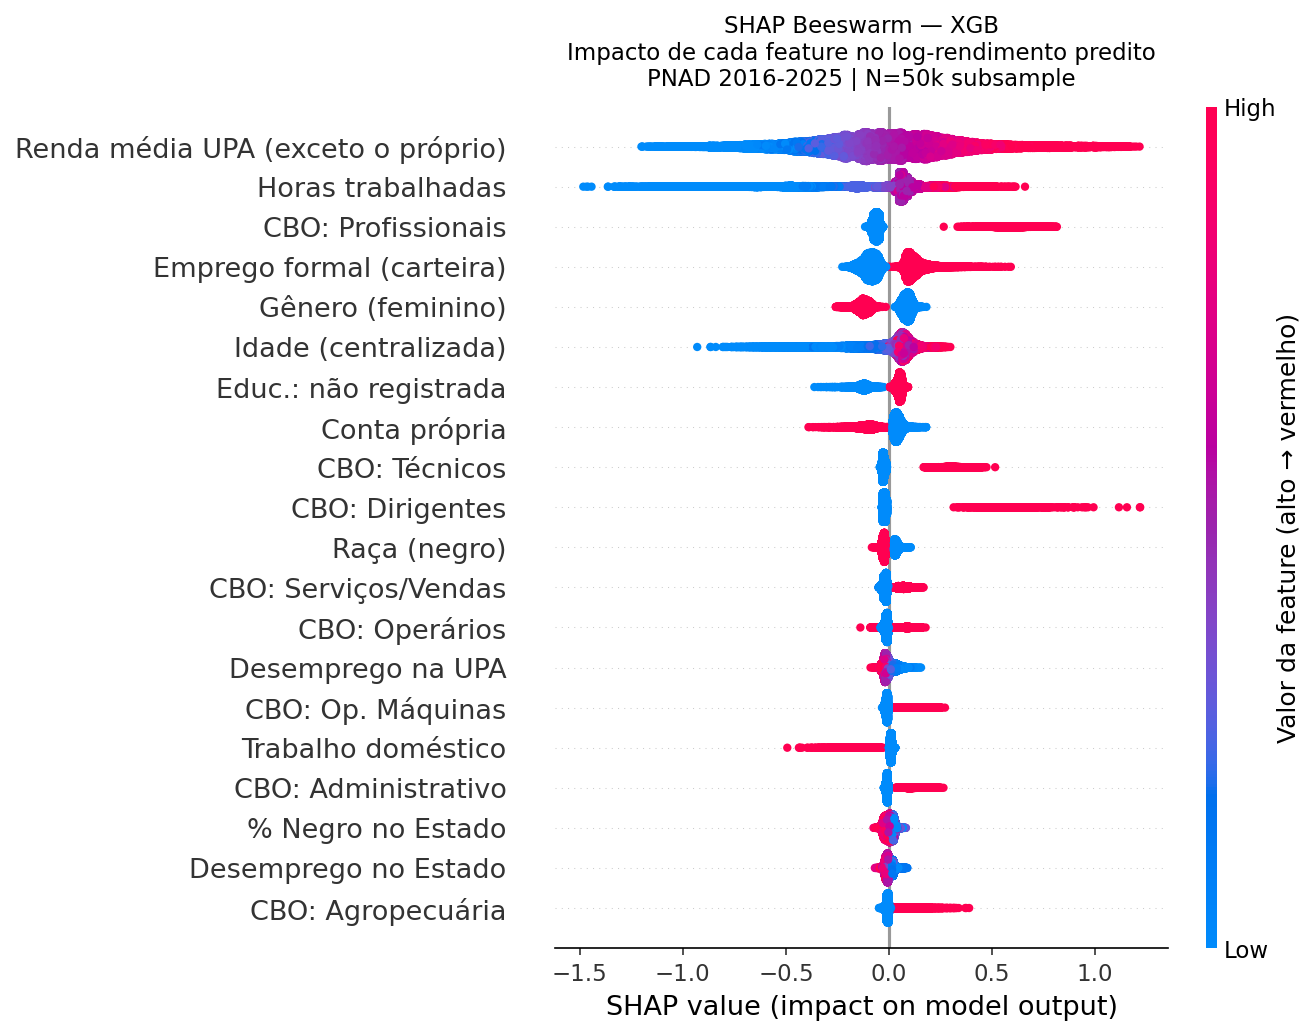
\includegraphics[width=0.92\textwidth]{shap_beeswarm_xgb}
  \caption{Contexto do bairro, diploma superior e jornada dominam a previsão de renda; a raça
  aparece na 14\textsuperscript{a} posição entre 28 preditores (SHAP, XGBoost,
  $N_\text{SHAP}=50.000$).}
  \label{fig:shap}
\end{figure}
\noindent{Como ler a Figura~\ref{fig:shap}:} cada ponto é um trabalhador; quanto mais à direita (ou maior a barra), maior o efeito da variável na renda prevista. A cor indica se o valor da variável é alto ou baixo.

A Tabela~\ref{tab:shap_importance} mostra o \textbf{contexto do bairro} entre os
preditores de maior peso do rendimento individual. A variável usada aqui é a renda
média da UPA {excluindo o próprio indivíduo} ({leave-one-out}): a média que
inclui a própria pessoa é mecanicamente correlacionada com seu rendimento --- o
problema do reflexo \cite{manski1993} --- e inflaria artificialmente a importância do
território. Mesmo sem essa contaminação, o bairro permanece entre os preditores de
primeira ordem, o que é consistente com a hipótese de \citeonline{wilson1987}; a
leitura correta, porém, é de {mediação} territorial --- choques comuns ao bairro
(mercado de trabalho local, transporte, redes) afetam todos os moradores --- e não de
efeito causal de um vizinho sobre o outro. Como checagem extrema, o mesmo XGBoost
estimado {sem qualquer} renda de vizinhança perde pouco poder preditivo
($R^2 = 0,632$ contra 0,644 do modelo completo) e, nele, a contribuição
média da raça é praticamente a mesma (0,029 contra 0,027 em
$|\text{SHAP}|$): o sinal racial não é um artefato da variável de contexto ---
muda apenas a posição relativa no {ranking},\footnote{15\textsuperscript{a}
de 27 variáveis no modelo sem renda de vizinhança, contra
14\textsuperscript{a} de 28 no modelo completo.} porque as demais
variáveis absorvem parte do que o território explicava.

A variável racial ocupa o 14$^\circ$ lugar no ranking de
importância mesmo após controlar por todos os demais fatores. A parcela do
rendimento predito que o modelo atribui à raça difere em
5{,}3\% entre trabalhadores negros e
brancos\footnote{Contribuição média da variável racial à previsão, com sinal:
$-0{,}0241$ log-pontos entre os negros e
$+0{,}0299$ entre os brancos (XGBoost,
$N_\text{SHAP}=50.000$; \texttt{shap\_negro\_por\_grupo.csv}). A média de um
grupo mede o desvio em relação à previsão média da base, que mistura os dois; o
que corresponde ao coeficiente racial das regressões é o contraste entre elas.}
--- o que resta depois de educação, experiência, gênero, contexto de moradia e
ocupação. O valor fica a 0{,}4 ponto percentual do {gap} estimado
pelo M4 hierárquico, que usa controles semelhantes (o XGBoost acrescenta a renda média do
bairro): um algoritmo que não
impõe forma funcional alguma chega perto do modelo linear, sinal de que o
achado não depende da especificação de Mincer.

Os dois modelos discordam quanto à raça, e a Tabela~\ref{tab:shap_importance}
mostra a discordância: no Random Forest ela cai para o
20$^\circ$ lugar, com contribuição média próxima de zero,
enquanto as demais variáveis têm peso semelhante nos dois. A diferença é de
arquitetura, não de dados. Cada árvore da floresta escolhe, em cada nó, a
variável de maior ganho entre todas as disponíveis; com a profundidade limitada
a dez níveis, uma variável de efeito pequeno perde essa disputa em todos os nós
e acaba nunca sendo usada. O {boosting} trabalha em sequência sobre o
resíduo: consumidas as variáveis de maior peso nas primeiras iterações, o que
sobra passa a ter estrutura racial, e as árvores seguintes chegam a ela. É por
isso que a leitura se apoia no XGBoost, que é também o de melhor ajuste --- e é
uma ilustração do que a literatura de {ensembles} chama de sensibilidade
do modelo à forma como o erro é decomposto. A Figura~\ref{fig:shap_wf} ilustra como a previsão de dois casos individuais é composta.

\begin{figure}[H]
  \centering
  \begin{subfigure}[b]{0.49\textwidth}
    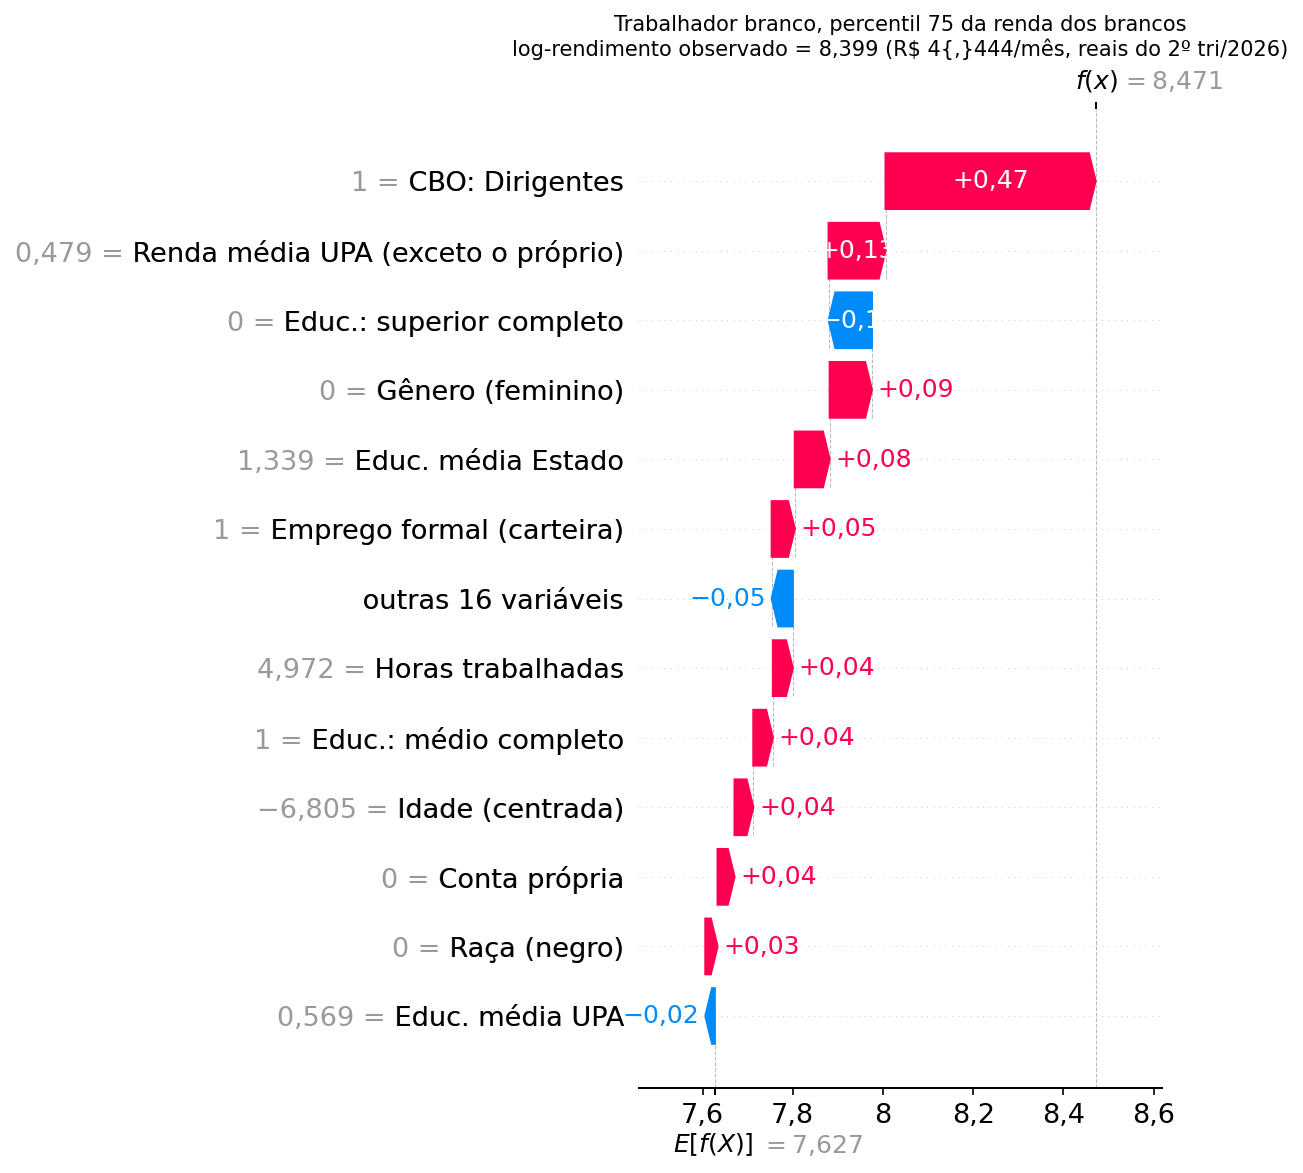
\includegraphics[width=\textwidth]{shap_waterfall_A_branco_alta_renda_xgb}
    \caption{Trabalhador branco.}
  \end{subfigure}
  \hfill
  \begin{subfigure}[b]{0.49\textwidth}
    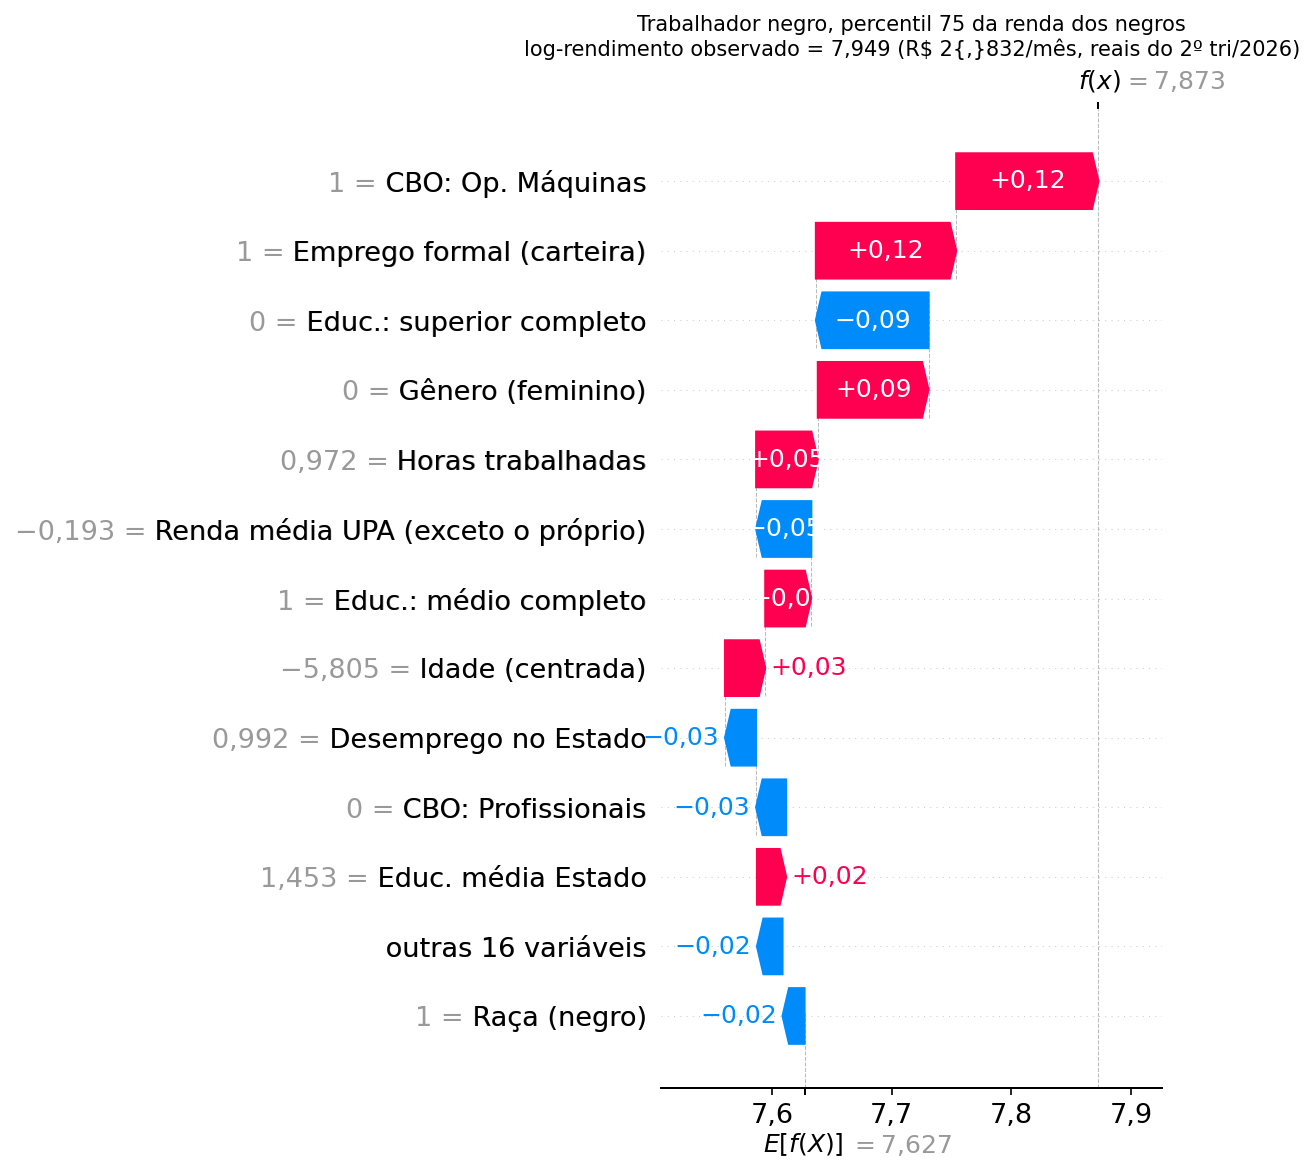
\includegraphics[width=\textwidth]{shap_waterfall_B_negro_alta_renda_xgb}
    \caption{Trabalhador negro.}
  \end{subfigure}
  \caption{A mesma variável, sinais opostos: a raça soma à previsão do
  trabalhador branco e subtrai da do negro. Decomposição SHAP individual
  ({waterfall}) de dois trabalhadores, cada um no percentil~75 de rendimento
  do próprio grupo; cada barra é a contribuição de uma variável ao afastamento entre
  a previsão média da base e a previsão daquele caso, em log-pontos, e as de menor
  peso estão agrupadas na linha das demais. Os painéis mostram como o modelo compõe
  uma previsão: a diferença de rendimento entre os dois é bruta, sem os controles
  que os modelos aplicam.}
  \label{fig:shap_wf}
\end{figure}
\noindent{Como ler a Figura~\ref{fig:shap_wf}:} cada linha é uma variável de \textbf{um} trabalhador --- não de uma média. A barra mostra quanto aquela variável empurra a previsão para cima ou para baixo, partindo da previsão média da base até a previsão final do caso. Compare a linha {Raça (negro)} nos dois painéis: é a mesma variável, com o sinal trocado --- soma no branco, subtrai no negro. Serve para ver como o modelo compõe uma decisão, não para generalizar: a magnitude média está na Figura~\ref{fig:shap}, sobre os 50 mil casos.

% ── NÚCLEO: decomposições e acesso (inserido pela versão enxuta) ──
\par
\medskip

\subsection*{Multicolinearidade do Modelo M4: Análise VIF}
Antes da Discussão, uma checagem técnica do modelo com mais controles, o M4. \label{subsec:vif}

Os controles do M4 estão brigando entre si? A pergunta é legítima: o modelo empilha nove indicadores de grupo ocupacional sobre três de vínculo, e variáveis muito próximas entre si inflam o erro-padrão umas das outras, a ponto de tornar instável justamente o coeficiente que interessa. O {Variance Inflation Factor} mede esse efeito: quanto a variância de cada estimativa cresce em razão das demais. A resposta, aqui, é que há colinearidade --- mas não onde ela importaria.\footnote{Calculado sobre a população completa da PEA com renda positiva. Dos $23$ preditores analisados, VIF máximo~$= 2,66$
(CBO: Profissionais); 0~variáveis críticas
(VIF~$> 10$); 0~variáveis altas ($5$--$10$);
6~variáveis moderadas ($2$--$5$);
17~variáveis baixas ($< 2$).}
Nenhum preditor do M4 tem VIF acima de 10; o maior é o de \texttt{ocp\_profissional} (2,66). A colinearidade que houver \textbf{não} contamina o coeficiente de
interesse: o VIF de
\texttt{negro} é 1,36 e o das variáveis de contexto da UPA fica abaixo de
2,2. Entre as {dummies} de CBO e as variáveis de vínculo --- a
colinearidade que se temia no M4 --- o VIF máximo é 2,66. A especificação
do M4 dispensa, portanto, ortogonalização ou eliminação de preditores; o que ela
não dispensa é a ressalva de {bad control} (Subseção ``Modelos Hierárquicos Lineares --- Mediação Contextual do Gap'').

\subsection*{Discussão}
\label{sec:discussao}

\paragraph{Nota terminológica.}
Três conceitos próximos, mas distintos, percorrem este trabalho e não devem ser
confundidos. \textbf{Mediação contextual} (HLM) é a fração do gap agregado
(condicional a capital humano e estado) que {desaparece} ao se compararem
pessoas do mesmo bairro (UPA) --- mede o quanto da penalidade racial transita
{pelo} território.
\textbf{Efeito dotação} (Oaxaca--Blinder) é a parcela do gap atribuível a
{diferenças nas características observáveis} entre brancos e negros
(escolaridade, ocupação, contexto), por oposição ao \textbf{efeito retornos}
(preços diferenciais pagos às mesmas características).
\textbf{Gap líquido} é o diferencial que {persiste} após o controle de
capital humano e contexto (M3): 6,1\%. \textbf{Gap residual pós-ocupação} é o
que resta ao se controlar também ocupação e formalidade (M4): 5,6\% --- um limite
inferior, pois a ocupação é ela própria resultado da barreira de acesso. Em suma: a mediação contextual responde
``por onde passa o gap''; a decomposição de dotações, ``de que ele é feito''; e o
gap líquido, ``o que sobra sem explicação''.

\paragraph{Da diagnose às políticas.}
O diagnóstico das duas barreiras revela gargalos simultâneos --- exclusão de
acesso às ocupações qualificadas e penalidade salarial que persiste dentro delas
--- que aparecem juntas nos mesmos dados. A consequência para o desenho de políticas
é direta: nenhuma intervenção unidimensional (só cotas de acesso, só fiscalização
salarial, só escolaridade) atinge as duas barreiras ao mesmo tempo; a magnitude
relativa de cada uma, estimada aqui, é o insumo para priorizá-las.

\paragraph{O que este trabalho acrescenta ao debate.}
\citeonline{hasenbalg1979} identificou a discriminação racial como estrutural,
sem poder quantificar mecanismos em escala nacional.
\citeonline{henriques2001} documentou o gap educacional racial, mas não separou
o efeito educacional do de redes e contexto.
\citeonline{soares2009} estimou, com dados de 2006, que cerca de 50\% do gap
salarial seria ``inexplicado'' --- interpretado como discriminação direta.
Este trabalho, com dados de 2016--2025 e metodologias não disponíveis
a Soares, decompõe essa {caixa preta}. Na especificação comparável à dele
(capital humano e contexto, sem ocupação), 17,9\% do gap bruto são retornos
diferenciais --- limite superior do tratamento diferencial --- e 82,1\% são
diferenças de dotações; quando a ocupação é tratada como dotação, o não explicado
cai para 15,4\%, e 84,6\% passam a ser dotações --- mas essas dotações são, elas mesmas,
produto da barreira de acesso às ocupações qualificadas (GLMM), que este
trabalho quantifica em conjunto com a penalidade salarial.
A contribuição central não é mostrar que o gap existe --- isso a
literatura já sabia desde \citeonline{hasenbalg1979} ---,
mas mostrar que ele é consistente com um
\textbf{sistema combinado} em que discriminação de acesso, segregação
residencial e penalidade salarial operam em conjunto, tornando
insuficientes políticas focadas em um único mecanismo.

\paragraph{Diálogo com o quadro macro recente do IBGE.}
Os resultados convergem com o retrato macroestrutural mais recente. A melhora multidimensional captada pela POF não eliminou o gap racial de qualidade de vida, e a renda voltou a concentrar-se no topo em 2025.\footnote{Índice de Perda de Qualidade de Vida (IPQV; quanto maior, pior) de 0{,}183 para chefes pretos ou pardos, contra 0{,}122 para brancos; Gini do rendimento domiciliar {per capita} de 0{,}491 em 2025 \cite{ibge_pof_2019, ibge_rendimentos_2025}.}
As duas medidas não são a mesma coisa, e a diferença importa para não se ler tendência onde há mudança de conceito.\footnote{O Gini estimado neste trabalho refere-se ao rendimento do trabalho entre ocupados (em torno de 0{,}47), ao passo que o do IBGE é domiciliar {per capita} e de todas as fontes. Os níveis são próximos, mas as medidas podem divergir em tendência: a alta de 2025 é puxada por renda não-trabalho do topo, que não transita pelo rendimento dos ocupados.} No conceito adotado aqui, a desigualdade {interna}
é maior entre brancos ($=0,477$) do que entre negros
($=0,436$) --- não por equidade, mas por confinamento dos
negros ao piso da distribuição, o reverso distribucional do teto de vidro.

\paragraph{Triangulação com o Índice de Progresso Social (IPS).}
O IPS municipal \cite{wilm2026} --- que avalia a qualidade de vida dos
5.570 municípios brasileiros a partir de 57 indicadores sociais e ambientais ---
oferece corroboração externa e multidimensional do eixo territorial desta tese.
Uma integração {fina} com o nosso proxy de bairro (UPA) é, contudo,
inviável: o painel público da PNAD não divulga o município (apenas UF e a situação
capital/RM/interior), e o IPS é municipal --- portanto mais agregado que a UPA, que
é sub-municipal. O IPS, assim, não valida o achado de {bairro}: situa-se
acima dele na escala e mede progresso social geral, não desigualdade racial. Fica
como agenda: com o município identificado (microdados de acesso restrito), seria
possível testar se a penalidade de bairro varia com o progresso social do município.


\paragraph{O diploma quase iguala o salário, mas não abre a porta.}
As duas barreiras respondem de modo diferente à escolaridade. A penalidade salarial é de 9{,}6\% entre quem não tem fundamental completo e cai a 1{,}1\% na pós-graduação (Figura~\ref{fig:hlm_negro_educ}); a desvantagem de acesso, não: com superior completo, as chances de um trabalhador negro chegar a um cargo qualificado seguem 18\% menores que as de um branco de mesmo perfil e bairro, e com pós-graduação, 23\% menores (GLMM, degrau A4, Tabela~\ref{tab:glmm_glassceil}). A escolaridade se associa a quase toda a convergência salarial, mas não à de acesso. Duas cautelas: são diferenças condicionais entre pessoas comparáveis, não o efeito de estudar mais --- quem chega à pós-graduação é um grupo selecionado ---, e as razões de chances do A4 incluem o vínculo, o que faz delas um limite inferior da desvantagem.

\paragraph{A segregação residencial como multiplicador da desigualdade.}
O achado mais robusto desta análise é que 39,5\% do gap salarial racial
condicional a capital humano é mediado pelo bairro de moradia --- muito além do que modelos
cross-sectionais típicos, que ignoram a estrutura aninhada dos dados,
seriam capazes de estimar. O coeficiente contextual
$\hat{\gamma}_{01} = −0,1272$ por desvio-padrão da proporção de negros na UPA
indica que a penalidade de viver em bairro segregado é da mesma ordem
de grandeza da própria penalidade individual de ser negro --- e que 35,3\%
da variância do rendimento está entre bairros, não entre pessoas.
Isso sugere que políticas de redistribuição de renda que não enfrentem
a segregação residencial terão eficácia limitada sobre o gap racial.

\paragraph{Subvalorização do capital humano negro.}
A decomposição de Oaxaca--Blinder atribui 17,9\% do gap a {retornos}
diferenciais --- as mesmas características de capital humano e contexto rendem
menos a trabalhadores negros --- e ainda 15,4\% quando a própria posição
ocupacional é descontada; a decomposição RIF mostra que essa parcela chega a 27\%
na base da distribuição. O GLMM acrescenta que a
credencial educacional não neutraliza a barreira de acesso (OR combinado de
\texttt{negro} de 0,818 entre os de superior completo). Juntas, essas evidências indicam
um duplo obstáculo ao retorno educacional: além da penalidade direta mensurada
pelo HLM, o acesso desigual às ocupações que convertem credenciais em renda.
\citeonline{granovetter1973} oferece o mecanismo plausível --- redes de indicação
que não cruzam fronteiras sociais ---, hipótese que este trabalho não testa
diretamente e que fica como agenda.

\paragraph{Persistência da discriminação direta.}
O gap líquido de 6,1\%, estimado após controlar por todos os vetores
de transmissão contextual, é o limite superior do intervalo --- cujo piso é o
M4, com a ocupação --- dentro do qual está a penalidade direta não explicada por
diferenças observáveis. Os valores SHAP reforçam essa
interpretação: a variável racial mantém o 14$^\circ$ lugar
na importância preditiva do XGBoost mesmo quando o modelo tem acesso
completo às variáveis educacionais, demográficas e contextuais.
Essa evidência é consistente com os experimentos de auditoria de
\citeonline{pager2007}, que demonstram experimentalmente a discriminação
racial em processos seletivos.

\paragraph{A convergência veio num degrau, e não num ritmo.}
Em dez anos o gap encolheu 14{,}7\%, e a inclinação é estatisticamente distinta de zero\footnote{$\delta = 0{,}000928$ log-ponto por ano, IC~95\% $[0{,}000133;\ 0{,}001723]$, $p = 0{,}027$, por mínimos quadrados ponderados sobre o $\hat\beta_{\text{negro}}$ do M3 estimado ano a ano, 2016--2025.}. Uma reta, porém, descreve mal a série. No estudo de evento --- a penalidade de cada ano contra a de 2019, com efeito fixo de bairro e erro agrupado por UPA, nível que difere do M3 por comparar só vizinhos ---, ela oscilou sem tendência de 2016 a 2019 e caiu em 2020, de 7{,}0\% para 5{,}9\% (1{,}0 log-ponto acima da tendência anterior, $p = 0{,}004$), sem voltar depois: em 2025 era de 5{,}2\%. A queda não reflete a saída dos negros de menor renda do emprego: a ocupação deles caiu só 0{,}26 ponto percentual a mais que a dos brancos em 2020, dentro da tendência anterior, e passou a crescer mais que a deles a partir de 2022, quando a penalidade seguia menor. Também não reflete a entrevista por telefone, adotada pelo IBGE em 2020 e 2021: a penalidade menor persistiu depois da volta da coleta presencial. Sem grupo de controle, a série não identifica a causa do degrau; ela mostra que a década não teve um ritmo de convergência a extrapolar, e que os resultados agrupados de 2016--2025 são uma média dos dois patamares. Nada disso trivializa os avanços recentes em políticas de cotas e de acesso ao ensino superior. Diz, sim, que reformas no campo educacional, sem intervenção simultânea nos mecanismos de segregação residencial e de acesso às ocupações, são insuficientes --- que é precisamente o que a sequência de modelos deste trabalho mostrou.


\paragraph{O que os resultados dizem sobre a política de diversidade vigente.}
\textbf{As políticas cuidam do ingresso, não da subida.} A reserva de vagas no ensino superior federal \cite{brasil2012lei12711, brasil2023lei14723} e nos concursos federais \cite{brasil2014lei12990, brasil2025lei15142} atua na entrada. A desvantagem medida aqui, porém, cresce onde se decide a ascensão: as chances de alcançar o décimo mais rico foram 24\% menores, e, entre os dirigentes, a mulher negra teve a menor chance de todos os grupos (OR~$=0,63$). O único instrumento federal voltado ao comando, a reserva de cargos em comissão e funções de confiança \cite{brasil2023decreto11443}, vale apenas para a administração pública federal, e o setor privado, que concentra a maior parte do emprego, não tem obrigação equivalente. O recorte por setor torna o diagnóstico mais preciso. Mesmo com reserva de vagas nos concursos desde 2014, o setor público não abre mais a porta do cargo qualificado (OR~$0,786$, contra $0,783$ no privado): a reserva opera na admissão ao serviço público, não no nível da ocupação, e os ocupados incluem coortes anteriores a ela. O que o setor público tem é um teto que pesa bem menos --- no décimo mais rico, $0,843$ contra $0,685$ --- e penalidade salarial menor (4,6\% contra 7,2\%). É no setor privado que a subida mais se fecha, o que é compatível com a ausência de obrigação, mas também com a estrutura salarial regulada do setor público; os dados não separam as duas leituras.

\textbf{A aposta educacional é necessária, mas insuficiente.} A escolaridade se associou a quase toda a convergência salarial --- a penalidade caiu de 9,6\% sem fundamental completo para 1,1\% na pós-graduação ---, mas não à de acesso: com pós-graduação, as chances de chegar a um cargo qualificado seguiram 23\% menores. Programas de acesso ao ensino atacam a barreira que mais cede ao diploma.

\textbf{Não há território na política de diversidade.} A diversidade é medida dentro da empresa, mas 39,5\% do diferencial agregado passou pelo bairro de moradia, e nenhum instrumento federal de diversidade usa o local de moradia como critério.

\textbf{Um eixo de cada vez deixa a mulher negra de fora.} Ela entrou mais do que o homem branco nas ocupações feminizadas --- apoio administrativo (OR~$=1,96$), ensino e saúde ---, mas menos do que a mulher branca (OR~$=2,20$ no apoio administrativo); metas separadas para mulheres e para negros podem ser cumpridas pela mulher branca e pelo homem negro sem alcançá-la. A lei de transparência salarial \cite{brasil2023lei14611} coleta raça no relatório das empresas com 100 ou mais empregados, mas a obrigação de igualdade que estabelece é entre mulheres e homens.

\paragraph{Propostas para reduzir o racismo estrutural no mercado de trabalho.}
As propostas a seguir são sugeridas pelos resultados, não avaliadas por eles. \textbf{(i) Metas de representação em cargos de direção e gerência no setor privado, com recorte interseccional}, apoiadas no relatório que a lei de transparência salarial já exige. \textbf{(ii) Igualdade salarial por raça como obrigação, e não só como dado}, com fiscalização dirigida à diferença que persiste dentro da mesma ocupação (5,6\%), base que a proibição de práticas discriminatórias e o Estatuto da Igualdade Racial já oferecem \cite{brasil1995lei9029, brasil2010lei12288}. \textbf{(iii) Um componente territorial}. Dos resultados decorrem três pontos: o bairro carrega parte do diferencial; a penalidade é maior nos bairros de renda mais alta, o que pede fiscalização também ali, e não só na periferia; e as estimativas por bairro do modelo hierárquico servem para escolher onde começar e para medir se a penalidade mudou. A literatura de efeitos de vizinhança \cite{wilson1987, sampson1997, marques2010} sugere os instrumentos: transporte e intermediação de emprego que liguem os bairros segregados aos polos de emprego qualificado; aprendizagem, estágio e mentoria que levem redes de contato a quem não as tem --- como a penalidade cresce com a idade, agir na entrada evita que ela se acumule, se a leitura de ciclo de vida for a correta ---; currículo sem endereço nas primeiras etapas de seleção; escola de tempo integral e ensino técnico nos bairros de maior proporção de população negra; e habitação de interesse social em áreas centrais. \textbf{(iv) Promoção, e não só ingresso}: estender a lógica da reserva de cargos de confiança às empresas estatais e à progressão nas carreiras. \textbf{(v) Monitoramento anual} destes indicadores --- o diferencial líquido, a chance de acesso e a chance de comando por raça e gênero ---, reproduzíveis com a PNAD Contínua, para verificar se uma intervenção moveu a barreira que importa.

\subsection*{Limitações e escopo de validade}

\paragraph{Natureza inferencial {vs.}\ preditiva dos modelos.}
Os resultados devem ser lidos sob dois regimes epistemológicos distintos.
Os modelos HLM, a decomposição de Oaxaca--Blinder, a regressão quantílica e
o modelo logístico de acesso produzem {estimativas de associação condicional}:
medem o diferencial racial que persiste após o controle de covariáveis
observáveis, sob o pressuposto de seleção em observáveis. Não constituem, por
si sós, prova de causalidade no sentido contrafactual, pois não derivam de
desenho experimental ou quase-experimental. Já o XGBoost e os valores SHAP têm
finalidade {preditiva e interpretativa}: quantificam a contribuição de
cada variável para a {previsão} do rendimento --- não o efeito causal
de manipulá-la. A convergência entre os dois regimes (a raça mantém importância
preditiva não desprezível {e} coeficiente negativo significante sob
controle exaustivo) é o que confere robustez ao diagnóstico; ainda assim, a
linguagem causal foi deliberadamente evitada.

\paragraph{Condicionar em quem tem renda positiva.}
Todos os modelos de rendimento são estimados entre ocupados com renda positiva. Isso é
{condicionar no desfecho} (\citeonline{angrist2009}, cap.~3): se a discriminação
também reduz a probabilidade de estar ocupado, o gap salarial condicional mistura o
efeito sobre o salário com a seleção de quem permanece na amostra. A direção provável do
viés é de {subestimação}: se os trabalhadores negros que conseguem se manter
ocupados são positivamente selecionados em atributos não observados, o gap entre os
observados é menor que o gap potencial na população. O modelo logístico de acesso trata
diretamente a outra metade do problema --- a probabilidade de chegar à ocupação
qualificada ---; uma correção de seleção à Heckman, que exigiria uma variável de
exclusão crível (algo que afete estar ocupado sem afetar o salário), fica como extensão
e não é estimada aqui. A leitura correta é, portanto: o gap líquido aqui reportado
é o gap {entre ocupados}, não o gap potencial de toda a população em idade ativa.

\paragraph{As hipóteses, uma a uma, e o que acontece se falharem.}
Seguindo a recomendação de ``ser o próprio cético'' (\citeonline{angrist2009}, cap.~8):
\begin{enumerate}
  \item \textbf{Seleção em observáveis (CIA).} O gap líquido só é o efeito do tratamento
    diferencial se, condicional a $X$, a raça for ``como se'' aleatória. Não é: qualidade
    da escola, habilidade não medida e redes ficam fora. Se esses omitidos correlacionam
    negativamente com ser negro e positivamente com renda, o coeficiente {superestima}
    a discriminação --- por isso o gap líquido é apresentado como limite superior dessa
    leitura, e o Konfound/E-value quantificam quanto de confundimento seria preciso.
  \item \textbf{{Bad controls}.} Ocupação e formalidade são desfechos da
    própria discriminação; a jornada, não: com renda mensal, ela é controle necessário
    e entra nas duas especificações da Oaxaca--Blinder --- no modelo de acesso, só no
    degrau de limite inferior. Com eles (M4, Oaxaca-Blinder de acesso) o resultado é um
    {limite inferior descritivo}: a parcela que opera pela porta de entrada some da
    conta. Sem eles (M3, especificação~(A) da Oaxaca-Blinder) tem-se o gap total
    condicional a capital humano e bairro. As duas versões são reportadas lado a lado.
  \item \textbf{Reflexo (Manski).} Uma média de bairro que inclui o próprio indivíduo é
    mecanicamente informativa sobre ele --- a raça da pessoa entraria no \% de negros do
    seu bairro. Por isso todas as médias de contexto, de UPA e de UF, são calculadas sem a
    própria observação ({leave-one-out}), e a renda média do bairro, a mais exposta ao
    problema, fica fora dos modelos estatísticos e só entra como preditor no XGBoost. Isso remove o reflexo mecânico, mas choques
    comuns ao bairro ainda impedem leitura causal do coeficiente contextual.
  \item \textbf{Efeitos aleatórios.} O HLM e o GLMM supõem que o efeito de bairro não é
    correlacionado com os regressores. Como contraprova, todos os coeficientes foram
    reestimados com efeitos fixos de UF e erro-padrão agrupado por UPA, com as mesmas
    conclusões (Subseção ``Inferência: erros-padrão agrupados, poucos clusters e pesos'').
  \item \textbf{Pesos e desenho amostral.} As estimativas são não ponderadas: descrevem a
    regressão na amostra. A robustez ponderada pelo peso da PNAD muda o gap em cerca de
    meio ponto percentual.
  \item \textbf{Correlação intragrupo.} Ignorá-la subestimaria os erros-padrão (Moulton);
    todos os modelos reportam erro-padrão agrupado por UPA ou o modelam por efeito
    aleatório, e o agrupamento por UF usa $t$ com $G-1$ graus de liberdade.
  \item \textbf{Significância com $N$ grande.} Com 7{,}7 milhões de observações, quase tudo é
    ``significativo''; a leitura privilegia magnitude, intervalos de confiança e E-values,
    não asteriscos.
\end{enumerate}

\paragraph{Desenho transversal e direções futuras.}
O caráter transversal do painel público impede a análise de trajetórias
individuais; o painel rotativo completo com microdado identificado e a extensão
à RAIS permitiriam investigar mobilidade e o teto de vidro em cargos de liderança
com identificação de firma. A análise de redes de co-residência, a tipologia
por agrupamento e a priorização de políticas por pesquisa operacional,
desenvolvidas em versão estendida deste trabalho, ficam como agenda. Também fica
como agenda o uso de texto livre: a PNAD divulga ocupação e atividade já codificadas
(CBO e CNAE Domiciliar), sem o relato aberto da entrevista, de modo que técnicas de
processamento de linguagem natural não têm aqui onde se aplicar. Bases que associam
texto a indivíduos --- descrições de cargo em registros administrativos, anúncios de
vaga e currículos, como nos experimentos de auditoria \cite{pager2007} --- permitiriam
medir o conteúdo das funções e a triagem na contratação, que os códigos ocupacionais
não captam. A descrição oficial dos códigos não supriria essa lacuna: seria a
ocupação de novo, um {bad control} no modelo de rendimento e o próprio desfecho
no de acesso. Fica ainda como agenda relacionar a penalidade estimada em cada estado
à presença de pretos e pardos nos cargos eletivos, que a Justiça Eleitoral registra
por cor ou raça desde 2014: a sub-representação negra no comando político seria a
face institucional do teto de vidro aqui medido \cite{almeida2019}, mas, com uma
observação por estado, a comparação seria apenas ecológica.

\bigskip



\subsection*{Declaração de uso de inteligência artificial}
Na elaboração deste trabalho foram utilizadas ferramentas de inteligência
artificial (Claude Code, da Anthropic) como apoio à implementação e depuração de
código (Python e R), à geração de figuras e tabelas e à formatação dos documentos.
A concepção da pesquisa, a escolha das metodologias, a interpretação dos resultados
e a redação final são de responsabilidade do autor, que revisou, validou e responde
por todo o conteúdo.

% ══════════════════════════════════════════════════════════════════════════════


\section*{Conclusão}

A desigualdade racial no mercado de trabalho brasileiro apresentou as marcas do racismo estrutural. Persistiu: com a mesma escolaridade, idade, sexo e bairro, trabalhadores negros ganharam 6,1\% a menos, e 5,6\% dentro da mesma ocupação. Passou por estruturas: o bairro mediou 39,5\% do diferencial agregado, e as chances de chegar a um cargo qualificado foram 19\% menores. Acumulou-se rumo ao topo: a penalidade condicional subiu de 4,3\% na base para 8,4\% no nono decil. A mulher negra entrou pelas ocupações feminizadas, mas foi o grupo com menor chance de chegar ao comando. A penalidade foi maior para pretos (7,4\%) que para pardos (5,8\%) e cresceu com a idade. O diploma quase igualou o salário (1,1\% na pós-graduação), mas não a porta: as chances de acesso seguiram 23\% menores. As três hipóteses encontraram respaldo.

Esses resultados indicam limites da política de diversidade vigente. As cotas atuam no ingresso, mas a desvantagem cresce onde se decide a ascensão. No setor público, a porta do cargo qualificado foi tão desigual quanto no privado; o teto pesou menos. A educação reduz a penalidade salarial, mas não abre a porta. O território não entra nos critérios, embora carregue parte do diferencial. Metas separadas por raça e por gênero não alcançam a mulher negra no comando. As prioridades sugeridas são metas de representação em cargos de direção com recorte interseccional, igualdade salarial por raça como obrigação fiscalizada, ação territorial nos bairros de maior proporção de população negra e monitoramento anual destes indicadores. Os resultados são associações condicionais, não efeitos causais, e as propostas são agenda, não efeito estimado.


\newpage
\bibliography{relatorio_tcc}
\bibliographystyle{abntex2-alf}

\end{document}
